    \section{Case Study: LIGO Data Analysis}

    The previous case study demonstrated an example of "Event-driven" topological signature identification on Tableau Super-Store Sales Data \cite{TableauSuperStore} with the help of unique filter-specific R-K Diagrams generated using the R-K pipeline. In this second case study, we aim to extend the identification of unique topological signatures with a classification use-case to address an important scientific problem in the field of Gravitational-Wave Astronomy, that has been exploding with research and interest in recent years. \cite{00.3_GravitationalWaveResearch}\cite{00.4_GWRevolution} Hence, we shall now demonstrate a more specialized and scientific application of the R-K pipeline on a  Physical Dataset (as elaborated in \hyperref[sec:PhysicalSystems]{section 4.2.1} with certain domain specific modifications intended for  Gravitational-Wave Analysis\cite{00.1_2012GWAnalysisFormalism} \cite{00.2_schutz2012GWDataAnalysis} on LIGO data, which would aid in the identification and classification of  Compact Binary Merger Events \cite{24.0_BinaryMergerIdentification} \cite{24.1_BinaryMergerClassify} such as Black Holes, Neutron Stars \& Candidate Primordial Black Holes. We have thus applied the R-K pipeline to data-strains and datasets released by the LIGO Open Science Centre \cite{01.5_LIGOOpenSci} \cite{00_LIGOOpenSciData} for the the successful demonstration of our computational framework.This dataset was specifically chosen over other scientific data for the following reasons:

    \begin{enumerate}
        \item {To extend the scope of our pipeline and demonstrate a classification use-case on a field of scientific research that would be both relevant and useful in modern day Astronomy}
        \item{To choose a cutting edge area of modern scientific research which involved very large volumes of data with high-dimensional features and properties spanning across multiple data-strains and datasets to prove that the core components of the R-K Work-flow can traverse and analyse such scientific case-studies with distinct advantages over traditional approaches}
        \item {To showcase the flexibility of the R-K pipeline with modifications necessary for specialised scientific study}
        \item{To demonstrate the ease, flexibility \& scalability of the R-K pipeline to extend its scope of applications on Multi-messenger Astronomy }
        \item{It is open-source and widely accessible to the scientific community for analysis and applications }
    \end{enumerate}

    \subsection{Methodology}
    The methodology of this implementation has been focused to address the following domain specific challenges specifically with respect to the classification of Compact Binary Event Merger signals pertaining to \textbf{\textit{Black Holes, Neutron Stars and Primordial Black-Hole (Dark Matter):}}

    \begin{enumerate}
        \item {Very long wave-forms}
        \item {Computational complexity}
        \item {Difficult to compress signature strain data and eliminate noise}
        \item {Difficult to new apply traditional techniques of machine learning and neural-networks over a wide variety of parameters and constraints or implement any theoretical or observational constraints to the same analytical model}
        \item {Standard Neural Nets \& ML Models cannot be used for classification due to lack of training data, templates and learning models}
        \item {Immense manual effort needed over moths of research and verification for Compact Binary Event Merger signal identification with no computational framework for the automated classification of Binary-Mergers}
    \end{enumerate}

    In order to obtain a holistic methodology for addressing the above challenges and constraints with respect to an efficient computational pipeline to ingest enormous amount of raw-data, segregate confident merger signals and then classify them into a particular category of compact objects (i.e. Black Holes, Neutron Stars, Primordial Black Holes etc.); it is important for us to segregate and specify different data sources for the purpose of our analytical framework. Therefore, the data under consideration has been divided into 3 categories along with its corresponding analytical procedures:
    \begin{enumerate}
        \item Primary Analysis which is carried out on Raw-Strain Data
        \item Secondary Analysis pertaining to the intrinsic physical properties of the compact binary coalescences
        \item Tertiary Data
    \end{enumerate}

    \subsection{Data Description}
    As mentioned in the previous section, the LIGO data was divided into 2 parts for primary and secondary analysis.

    \subsubsection{Primary Data Analysis}

    We can define Primary Analysis on LIGO data as follows:
    The Primary dataset consisted of strain data with the following information

    \begin{itemize}
        \item the interferometer photodiode output of each detector produces gravitational-wave strain data as a time series sampled at 16384 Hz for LIGO data.
        \item For the Advanced LIGO detectors, the calibration is valid above 10 Hz and below 5 kHz.
        \item The detectors also record hundreds of thousands of auxiliary channels, time series recorded in addition to the strain signal, that monitor the behaviour of the detectors and their environment.
        \item Strain data is down-sampled to 4kHz from the original 16 kHz to reduce the size of LOSC files while (arguably) losing no science content, since the higher frequencies are dominated by
        optical noise.
        \item Thus, a 4,096-second file contains 16,777,216 GW-strain samples from a single
        detector, represented as floating-point "doubles" (eight bytes each).
        \item Invalid data due to detector malfunction, calibration error, or data acquisition problems are
    tagged so that they can be removed from analyses.

    \end{itemize}

    Any descriptions pertaining to the above dataset will be referred to as \textbf{\textit{"Primary Data"}} in this paper.

    \subsubsection{Secondary Data Analysis}
    We can define Secondary Analysis on LIGO data as follows:
    The Secondary analysis was carried out on tabular data  on the intrinsic physical parameters of compact binary mergers using Bayesian Methods of Parameter Estimation. \cite{00.7_LIGOBayesianAnalysis} \cite{00.6_LIGOAnalysisPipeline} \cite{24.4_CompactBinaryParameterEstimates} \cite{24.5_GWParameterEsitmation} \cite{24.6_LIGOParameterEstimates} consisting of the following information:

    \begin{itemize}
        \item The most important information w.r.t. secondary analysis are the merger event labels on the Gravitational Wave Transient Catalogue as they would serve as the parent node in correspondence with their GPS merger times. \cite{00_LIGOOpenSciData} \cite{00.2_schutz2012GWDataAnalysis} e.g. Event Names : GW150914 \& GW 170817 corresponding to GPS times of 1126259462.4 \&  1187008882.4 respectively.
        \item The tabular data consisted of Mass (1) $(M_1)$, Mass 2 $(M_2)$, Network SNR, Distance (Mpc), $\chi_eff $ , Inspiral, Final Spin, Total Mass $(M_\odot)$, Chirp Mass $(M_\odot)$, Detector Frame Chirp Mass $(M_\odot)$, Final Mass $(M_\odot)$, Redshift $(Z)$, False Alarm Rate and (yr-1) Pastro  measures.
        \item However, due to the current sensitivity issues and LIGO VIRGO constraints \cite{24.8_PBHdetectionparameters} our analysis of compact binary classifications was primarily done between black holes, neurton stars and primordial black holes based on mass, spin, q-value ratios and red-shift measures with electromagnetic counterparts being added from Multi-messenger sources for further distinction of Neutron Stars w.r.t. Kilonova events that was left out of scope due to our focus on LIGO data in the initial version of this computational framework.
        \item Hence based on the ontological clustering of dependent and independent clusters the R-K models pertaining to secondary analysis of LIGO Data consisted of 4 independent clusters of Mass, Spin, Q-value ratios (derived from $(M_1)$ \& $(M_2)$)  and Red-shift.
        \item The following 4 events: GW170729, GW170817, GW190521 \& GW190814 in the chronological order of their GPS times, were chosen with some unique characteristics of mass, spin and q-values to demonstrate our methodology before executing the pipeline on the entire transient catalogue.

    \end{itemize}

    Any descriptions pertaining to the above dataset will be referred to as \textbf{\textit{"Secondary Data"}} in this paper.

    \subsubsection{Tertiary Data Analysis}
    We can define Tertiary Analysis on LIGO data as the data that is obtained from carrying our mathematical transformations on the secondary data there by giving rise to parameter specific refined measures such as q values, calculation of the evolution of the inward spiral and other measures obtained from theoretical analysis by applying mathematical equations to further evaluate and refine those parameters obtained using secondary analysis.

    \subsection{Objective of Analysis}

    To obtain unique event specific R-K diagrams and to showcase classification of Binary Event Mergers with high Signal to Noise Ratio (SNR) into a particular category of compact objects such as Black Holes, Neutron Stars or Primordial Black Hole Dark Matter.

    Modifications to the R-K pipeline have been done to signify confident binary merger signals and to use them as templates in combination with specific parameters and threshold filters to segregate such signals form false positives and detector noise in future. Furthermore, we have also endeavoured to provide a feasible computational pipeline that would enable the identification and classification of such binary mergers into specific category of compact objects based on secondary data analysis i.e. data obtained after on the various intrinsic physical parameters of such compact objects under consideration. Such secondary analysis is not carried out on Primary (Raw-Strain Data) but on secondary data Bayesian inference to calculate the posterior probability distribution over the parameters (sky location, distance, and/or intrinsic properties of the source) given the observed gravitational-wave signal.

    \subsection{Lens Implementation}

    As established earlier the choice of lens is critical for the basis of ontology and the R-K Model. Hence a binary coalescence or a compact binary merger event was chosen as the primary lens in this case study. Thus all parent nodes of of R-K diagrams on LIGO data would be represented by the binary-merger event label e.g. GW150914 (a typical BH-BH merger famously recorded in September 2015). Moreover, all central Event nodes pertaining to the "merger-event-lens" will also correspond to their respective GPS merger times in phase-space for the classification and analysis of R-K diagrams that are generated from R-K models build upon the choice of this lens. Furthermore, each attribute representing a characteristic physical parameter associated to a parent node or merger event would have a structural ontology with independent physical variable clusters such as all mass measures (M) and all spin parameters (S) clustered together with their dependent attributes such chirp mass, effective spin etc. as explained in section \ref{sec:PhysicalSystems}
    the unique attributes associated with such events would thereby serve as the  foundation for each R-K Diagram in this LIGO data analysis case study.

    \subsection{Preprocessing}

    As the current pipeline uses secondary measures, the preprocessing steps involved in the pipeline was naive. We ingested the secondary data into the pipeline and processed. In future versions of the LIGO R-K Pipeline, the process is intended to be much more elaborate, and eventually involving Bayesian Parameter Estimation over Primary Data as a means of feature extraction.

    \subsection{Modifications to the R-K Pipeline}

    We implemented a standard R-K Pipeline, with 2 stages for optimization. The first stage, involves generating unique topological signatures via a similar method to the store sales data. Training is done to maximize divergence using the same optimization objective function described in the Store Sale's \hyperref[sec:ObjectiveFunction]{Objective Function}.

    After optimization, we encoded the R-K Diagram into a vector and trained an SVM over the vectorized diagrams to produce a binary classifier over the data where X represents each vectorized R-K Diagram and Y are labels of PBH Merger events. Thus the pipeline required two levels of optimization.

    1. Embedding Optimization
    2. Classification Optimization

    \begin{figure}[H]
        \centering
        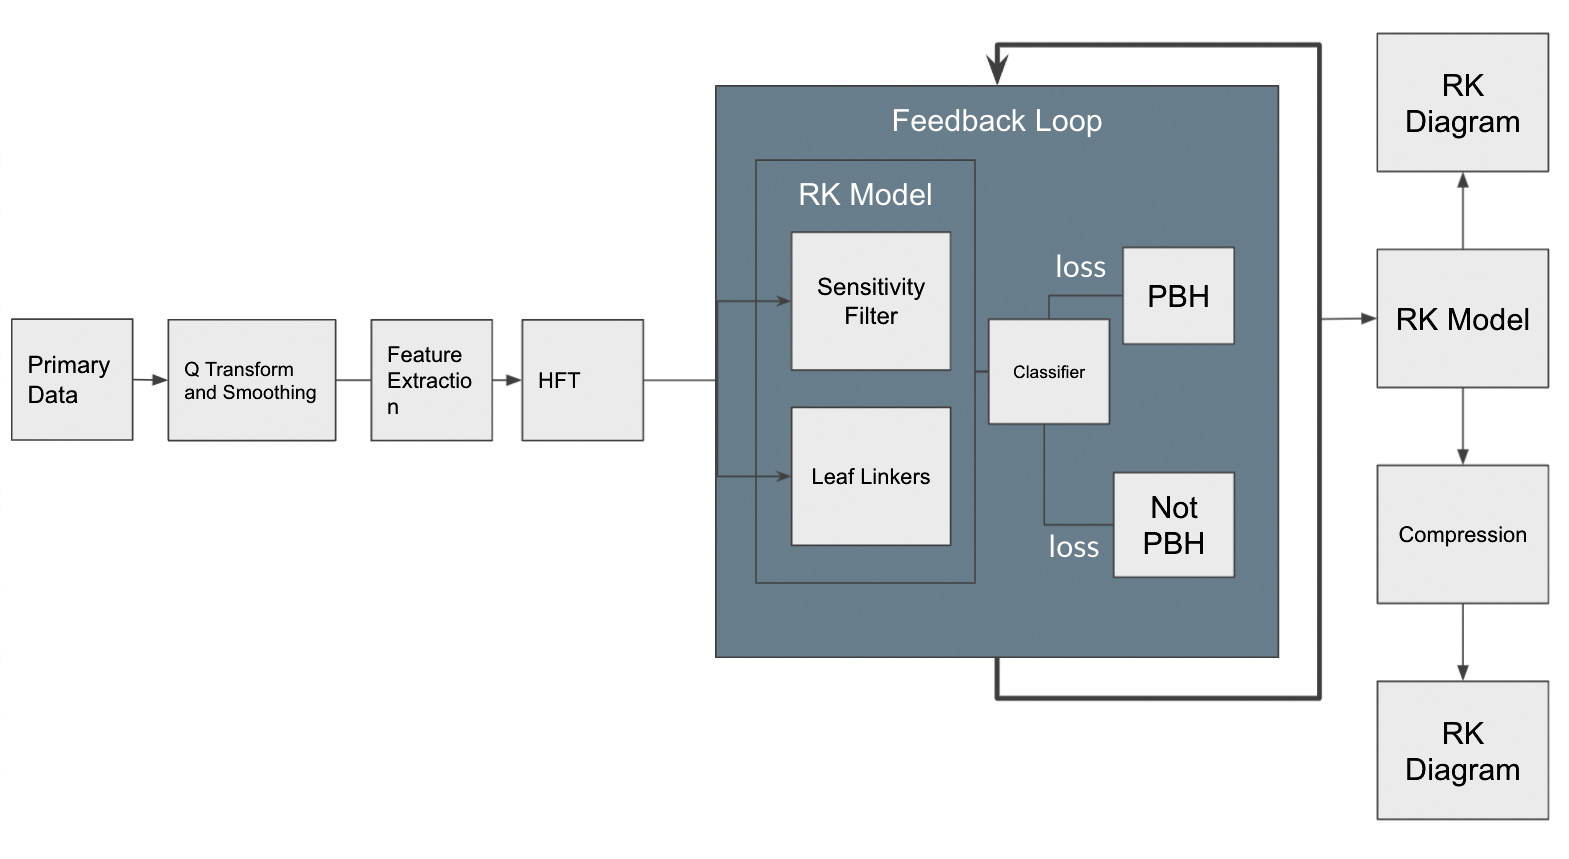
\includegraphics[width=1.0\linewidth]{images/ligo_pipeline.jpg}
        \caption{\textit{R-K Pipeline Modifications for LIGO Data Analysis}}
        \label{fig:ligo_pipeline_fig}
    \end{figure}

    These two optimizations, applied sequentially after each-other provide two artefacts:

    1. An R-K Pipeline which generates an R-K Diagram from a single event node
    2. An SVM Classification Boundary to which the R-K Diagrams can be applied against.

    We achieved R-K Diagram vectorization in a similar way to how a Bag of Words vectorization would be applied, where the ``corpus'' is all possible edges for a particular structural graph.

   \subsubsection{Modification Objectives}
    These modifications to the R-K pipeline were primarily motivated due to the address the following objectives:
    \begin{enumerate}
        \item To serve as a comparative classification frame-work for generating R-K Diagram based templates to classify and categorize compact-binary mergers with an efficient automated pipeline.
        \item To associate unique R-K Diagram classifications having distinct graph and topological properties with their  corresponding amplitude spectral densities (ASD) to allow for unique merger signal classification and segregation based on confidence scores of their corresponding R-K Diagrams in future.
        \item To enable a complete and holistic plug-and play computational framework linked directly to  primary data obtained from the detectors at source followed by effective filtering, noise reduction, Bayesian Parameter Estimation, deriving intrinsic physical parameters to build corresponding R-K models and applying filters and compressors to render the final R-K diagrams.
        \item These R-K diagrams could then serve as feedback templates generating more machine learning templates to optimize loss and refine binary merger signal classifications with further distinction.
    \end{enumerate}

    \subsection{Primary Data Analysis}

    Understanding the noise is crucial to detecting gravitational-wave signals and inferring the properties of the astrophysical sources that generate them. Improper modelling of the noise can result in the significance of an event being incorrectly estimated, and to systematic biases in the parameter estimation. To guard against these unwanted outcomes, detector characterization and noise modelling are significant activities within the LVC.\cite{00.5_GWDetectionNoiseCatalogue} While many textbook treatments of gravitational-wave data analysis describe the idealized case of independent detectors with stationary, Gaussian noise, actual LVC analyses are careful to account for deviations from this ideal.\cite{00.1_2012GWAnalysisFormalism} \cite{00.3_GravitationalWaveResearch}

    The Advanced LIGO and Advanced Virgo detector data have a rich structure in both time and frequency. For a given gravitational-wave source, the noise (as described by its spectral density) governs the measured signal-to-noise ratio (SNR). The spectral frequency content of the LIGO-Livingston detector was averaged over a three-minute period shortly before the first detection of gravitational waves from a binary neutron star merger with the event name GW170817.\cite{00.5_GWDetectionNoiseCatalogue}

    The steep shape at low frequencies is dominated by noise related to ground motion. Above roughly
    $100 Hz,$ the Advanced LIGO detectors are currently quantum noise limited, and their
    noise curves are dominated by shot noise. High amplitude noise features are also present in the data at certain frequencies, including lines due to the AC power grid (harmonics of 60 Hz in the U.S. and 50 Hz in Europe), mechanical resonances of the mirror suspensions, injected calibration lines, and noise entering through the detector control systems. \cite{00.1_2012GWAnalysisFormalism} \cite{00.5_GWDetectionNoiseCatalogue} \cite{00.3_GravitationalWaveResearch}

    \subsubsection{Strain Data}

    The R-K pipeline was retrofitted to run additional precursor steps on strain data as explained in the previous section. This is mainly done as a part of the additional component steps added to the R-K pipeline for reasons explained in section 6.6. The figure below demonstrates plotting of the raw data-strains with initial filters as explained. This process was then extended for all 4 selected events for the purpose of initial analysis and validation, namely:  GW170729, GW170817, GW190521 \& GW190814. The purpose of choosing all 4 events in parallel was done to demonstrate their eventual representations on an expanded topological "Event-scape" that would spread across a plane of GPS times and merger frequencies for all the events plotted together for the sake of future comparison.



    \begin{figure}[H]
        \centering
        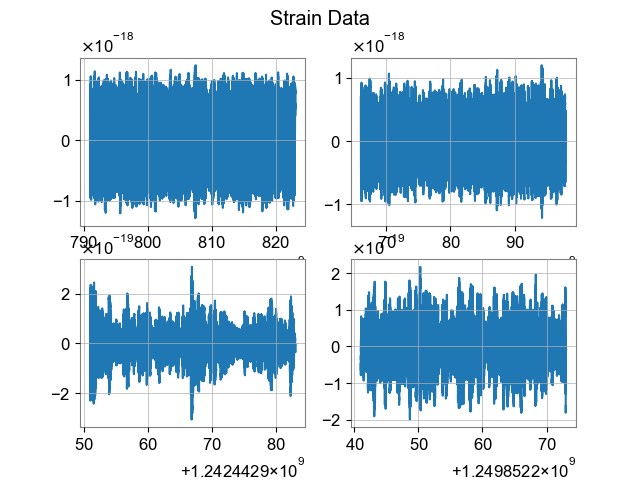
\includegraphics[width=1.0\linewidth]{images/44_01_Raw Strain Data.png}
        \caption{\textit{Raw Data Strain from LIGO}}
        \label{fig:LIGO1_PlaceHolder_fig}
    \end{figure}
    A sequence of processing steps was applied in our modified pipeline to the calibrated strains from the LIGO-Hanford detector such as the one showing $4 s$ of data centered on GPS time 1126259462 \(September 14, 2015 09\:50l\:45 UTC\). This data was obtained form the GW Open Science Center \cite{00_LIGOOpenSciData}. First a Tukey Window with $0.5 s$ is applied, then the data are whitened using an estimate of the noise spectral density. Finally the data are bandpassed filtered to enhance features in the passband (35 Hz; 350 Hz), there by revealing the presence of gravitational-wave signal $GW150914.$ This was done as a first trial run using the modified R-K pipeline in accordance with well established research papers. \cite{00.2_schutz2012GWDataAnalysis} \cite{00.5_GWDetectionNoiseCatalogue}
    The process described in the research papers were then applied to all 4 selected event stains obtained from the GW Open-Science Center and to showcase the capability of our computational framework in terms of processing primary and secondary data with respect to multiple compact binary-merger events in parallel.


    \subsubsection{Spectrograms \& Q-Transforms}

    It was seen that the raw or primary data from the previous stage are dominated by low-frequency noise. Therefore a  Tukey window with 0.5 s transition regions was applied to the raw data. Next, the data-stains were all whitened by dividing the Fourier coefficients by an estimate of the amplitude spectral density of the noise, which ensures that the data in each frequency bin has equal significance by down-weighting frequencies where the noise is loud. The data-strains were were then inverse Fourier transformed to return to the time domain using the following relation:
    \begin{equation}
      d(t) \stackrel{\mathrm{FFT}}{\longrightarrow} \tilde{d}(f) \stackrel{\text { Whiten }}{\longrightarrow} \tilde{d}_{w}(f)
    \end{equation}
    \begin{equation}
      \tilde{d}(f) \stackrel{\text { Whiten }}{\longrightarrow} \tilde{d}_{w}(f) =
      \frac{\tilde{d}(f)}{S_{n}^{1 / 2}(f)} \stackrel{\mathrm{iFFT}}{\longrightarrow}d_{w}(t)
    \end{equation}
The above bandpass technique enhances the visibility of features of interest in this band by removing noise outside of the band - seismic and related noise at low frequencies, and quantum sensing noise at high frequencies. However, it is important to note that Note that such narrow band-passing is only used for visualization purposes and is not employed in the LVC analyses.

    However, as indicated in LIGO research \cite{00.2_schutz2012GWDataAnalysis} \cite{00.3_GravitationalWaveResearch} \cite{00.6_LIGOAnalysisPipeline} \cite{00.5_GWDetectionNoiseCatalogue} Wavelets provide a more
    flexible analysis framework than short-time Fourier transforms. Continuous wavelet transforms are commonly used in LIGO-Virgo data studies to produce spectrograms that provide a visual indication of non-stationary behaviour. Quantitative assessments of non-stationary may also be made by using discrete, orthogonal wavelet transforms. This can be visualised in the best way using normalized q-transforms on the strain data by plotting the noise reduced data strain frequencies against GPS time in a 2-D plane with the normalised energy representing the amplitude spectral densities of each merger-event in the form of the combined plots shown below.

    \begin{figure}[H]
        \centering
        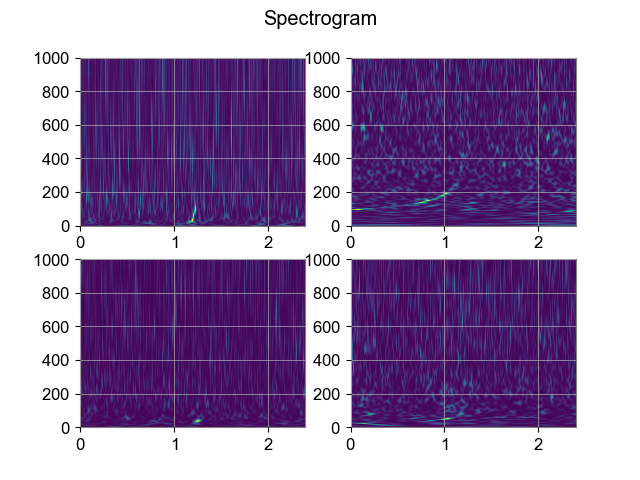
\includegraphics[width=1.0\linewidth]{images/46_03_LIGO Spectograms with Q Transformed ASD.png}
        \caption{\textit{LIGO Spectrograms with Q Transformed ASD}}
        \label{fig:LIGO Spectograms with Q Transformed ASD}
    \end{figure}

Here the normalised energy  of the Q-transform coefficients can be calculated using the following relation:

\begin{equation}
	E=\frac{|X(\tau, \phi, Q)|^{2}}{\left\langle|X(\tau, \phi, Q)|^{2}\right\rangle}
\end{equation}
Thus, the Q- transform pipeline can be thought of as an optimal matched filter search for minimum uncertainty waveforms of unknown phase in the whitened data streams.

    \subsubsection{Topological Event Scape}

    However, we found that the true power of topological analysis could be utilised in the best way possible by merging all events in 3D for shape rendering and signal filtration using noise reduction techniques. This notion is inspired by topological data visualisation techniques which increase the granularity and bring out the details within high dimensional datasets for further distinction and analysis.

    \begin{figure}[H]
        \centering
        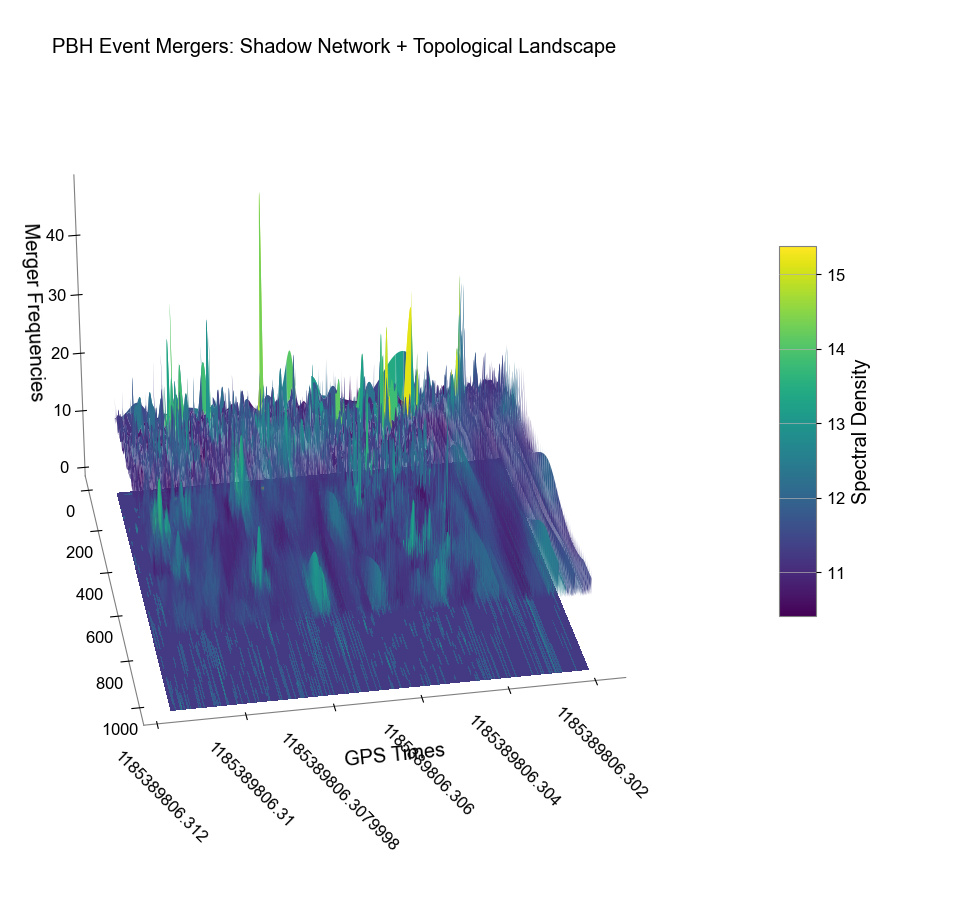
\includegraphics[width=1.0\linewidth]{images/48_05_Topo Transformed Eventscape with Phase Projected Network.jpg}
        \caption{\textit{3D Projected Event-scape with spectral density map of combined events and Phase Projection of Event Signatures according to GPS Time \& Frequency}}
        \label{fig:LIGO3_PlaceHolder_fig}
    \end{figure}

    Thus, the above diagram shows a "Topological Event-Scape" of all 4 merger events with GPS times and merger frequencies representing the 2 axes of the 2D plane while the amplitude of the spectral density representing the normalised energy is plotted in the 3D dimension to bring about more enhanced filtering and noise reduction around the Tukey window with appropriate filters.This is also made possible by the fact that all mergers can be combined together and compared with each other using Universal GPS times and because all mergers tend to have their Fourier transformed frequencies within a comparative scale of values.

    \subsubsection{Filtration \& Noise Reduction}

    In this section we outline how we identify and characterize these noise features so that we can either exclude the bad data or assess the impact of remaining components to search for gravitational-wave signals. This concept can be further enhanced to all data-strains in parallel using the R-K pipeline as shown and can be extended to 'n' number of events in theory. However, we have addressed our 4 selected events  GW170729, GW170817, GW190521 \& GW190814 for the sake of simplicity and clarity.

    In this pipeline, noise reduction filters could be applied to all events simultaneously and we used a combination of Gaussian filters and cosine based Tukey filters such as the one defined below:

    \begin{equation}
        w(x)= \begin{cases}\frac{1}{2}\left\{1+\cos \left(\frac{2 \pi}{r}[x-r / 2]\right)\right\}, \& 0 \leq x<\frac{r}{2} \\ 1, \& \frac{r}{2} \leq x<1-\frac{r}{2} \\ \frac{1}{2}\left\{1+\cos \left(\frac{2 \pi}{r}[x-1+r / 2]\right)\right\}, \& 1-\frac{r}{2} \leq x \leq 1\end{cases}
    \end{equation}

    \begin{figure}[H]
        \centering
        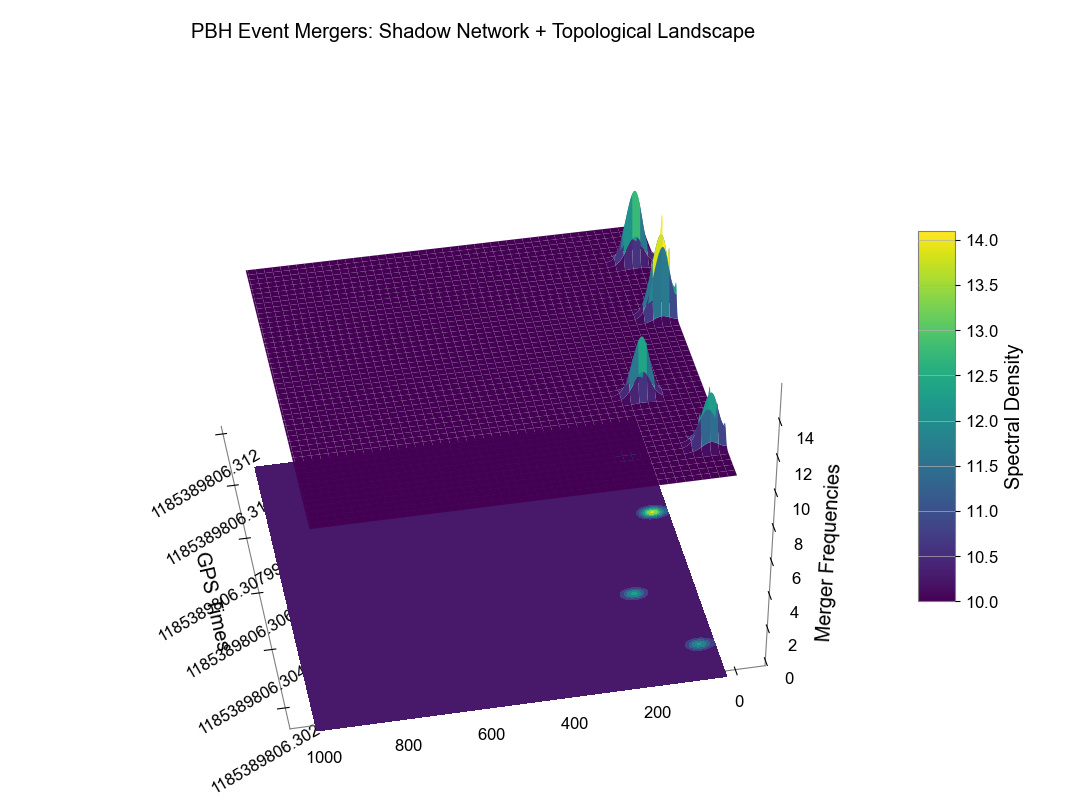
\includegraphics[width=1.0\linewidth]{images/49_06_Topological Noise Reduction on Primary data with phase prijections.jpg}
        \caption{\textit{Topological Noise Reduction on Primary data with phase projections}}
        \label{fig:LIGO4_PlaceHolder_fig}
    \end{figure}

    This allowed us to achieve significant noise elimination while preserving the essential frequencies and spectral energy densities of the merger signals about their corresponding GPS times which could also be reverified using established secondary data from LIGO, thereby establishing the validity of this technique as shown in the above diagram.

    Furthermore, our computational framework allowed for the visualization and mapping of the peak frequency of the 3D wave spectral densities to their corresponding GPS time stamps using phase projection techniques described in the mathematical formalism of this paper.

    \subsubsection{Phase Projections}

    The Phase space projections of the peak frequencies of noise-reduced and filtered gravitational wave merger signals not only correspond to their GPS merger times but is very useful to serve as the choice of lens to build R-K models with  secondary attributes and parameters clustered about these primary event nodes as we shall see in the following sections of this paper.
    \begin{figure}[H]
        \centering
        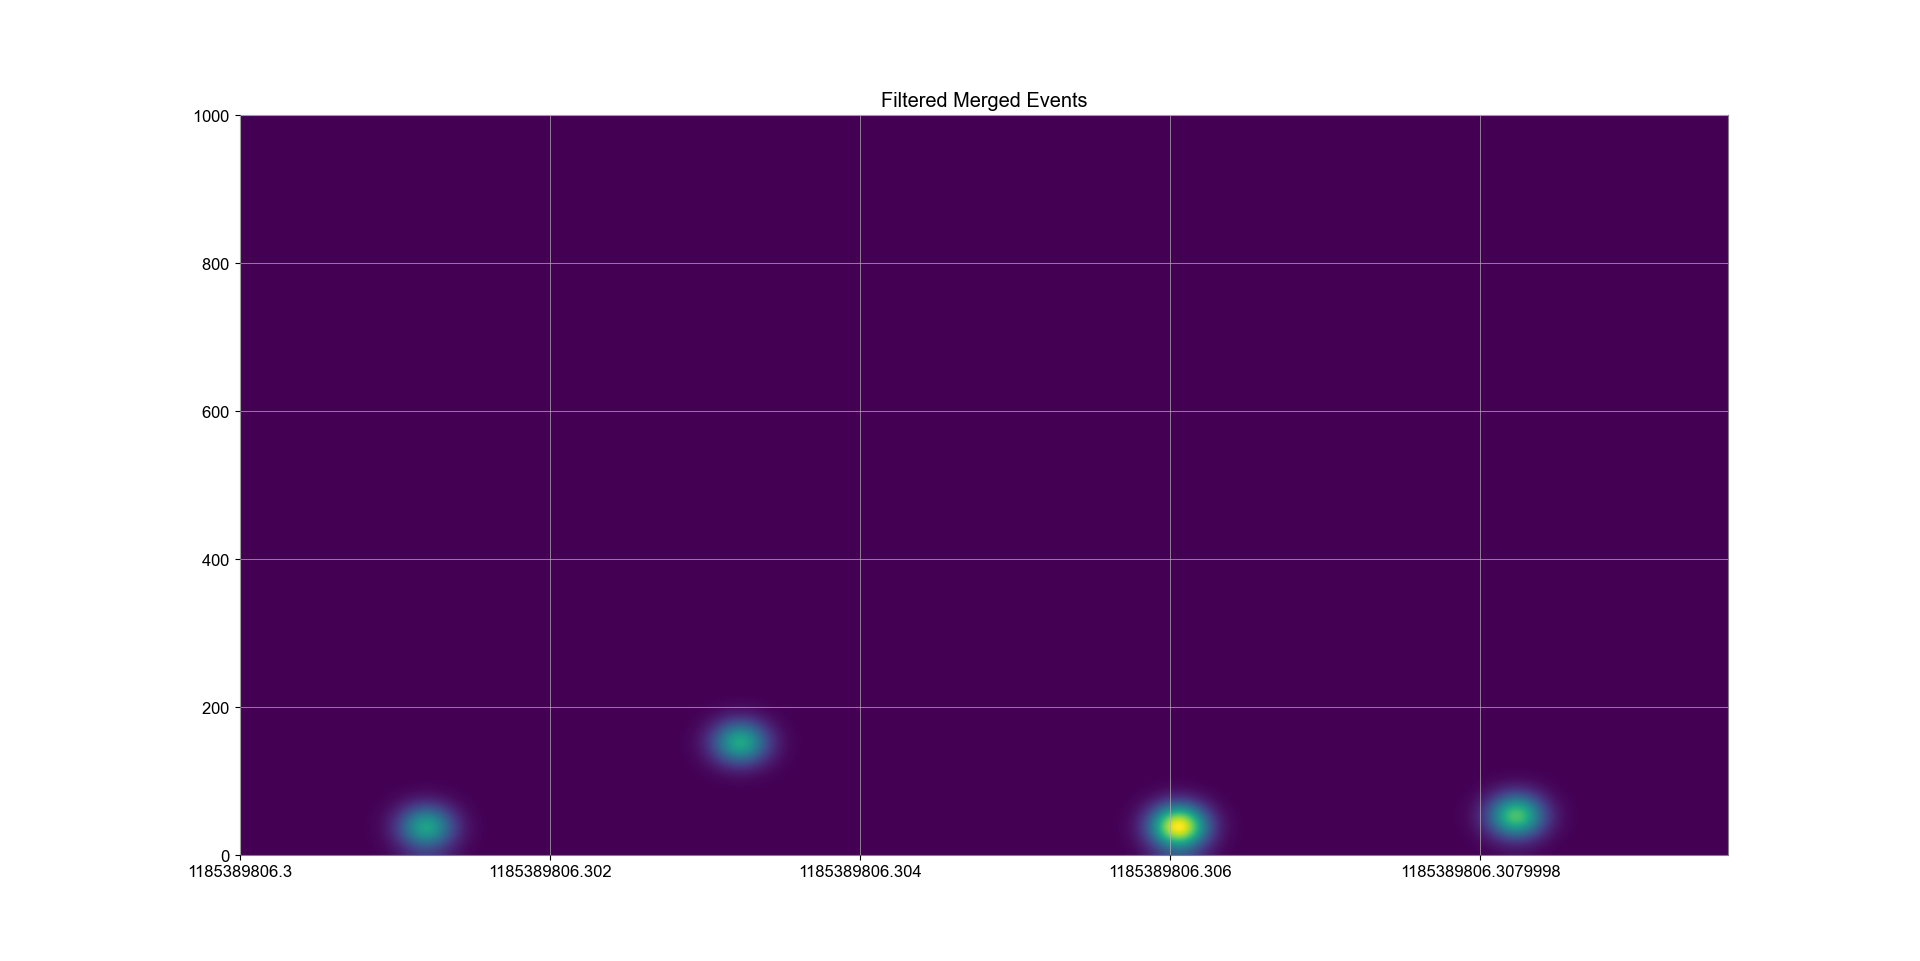
\includegraphics[width=1.0\linewidth]{images/50_07_Phase Projections of Noise Reduced Topological Merger Signals.png}
        \caption{\textit{Combined Phase Projections of Noise Reduced Compact Binary Merger Signals}}
        \label{fig:LIGO5_PlaceHolder_fig}
    \end{figure}

    \subsection{Secondary Analysis}

    We shall now extend the pipeline with the  exploration of secondary measures obtained using posterior probabilities and Bayesian parameter estimates in established research. \cite{24.0_BinaryMergerIdentification} \cite{24.4_CompactBinaryParameterEstimates} \cite{24.5_GWParameterEsitmation} \cite{24.6_LIGOParameterEstimates} It is however, important to note that the current version of the LIGO R-K pipeline does not address the computation of posterior probabilities and Bayesian parameter estimates from Primary Data. This remains to be in the scope of future research which could potentially help automate this entire process thereby generating R-K diagrams directly from detector signal data in near-real time and classifying them into a specific category of compact objects such as Black Holes, Neutron Stars, Primordial Black Hole Candidates etc.

    However, for the sake of the first version of the computational framework and R-K pipeline, we have restricted the scope of this paper in carrying out Secondary Analysis on the estimated physical measures corresponding to each merger event as published. \cite{00_LIGOOpenSciData} \cite{00.7_LIGOBayesianAnalysis} \cite{00.6_LIGOAnalysisPipeline}

    \subsubsection{Omni-view Plots}

    Thus using the flexibility and scalability of the R-K pipeline we have plotted an "Omni-view Plot" of all secondary measures plotted against each other with respect to the entire GWTC currently available.

    \begin{figure}[H]
        \centering
        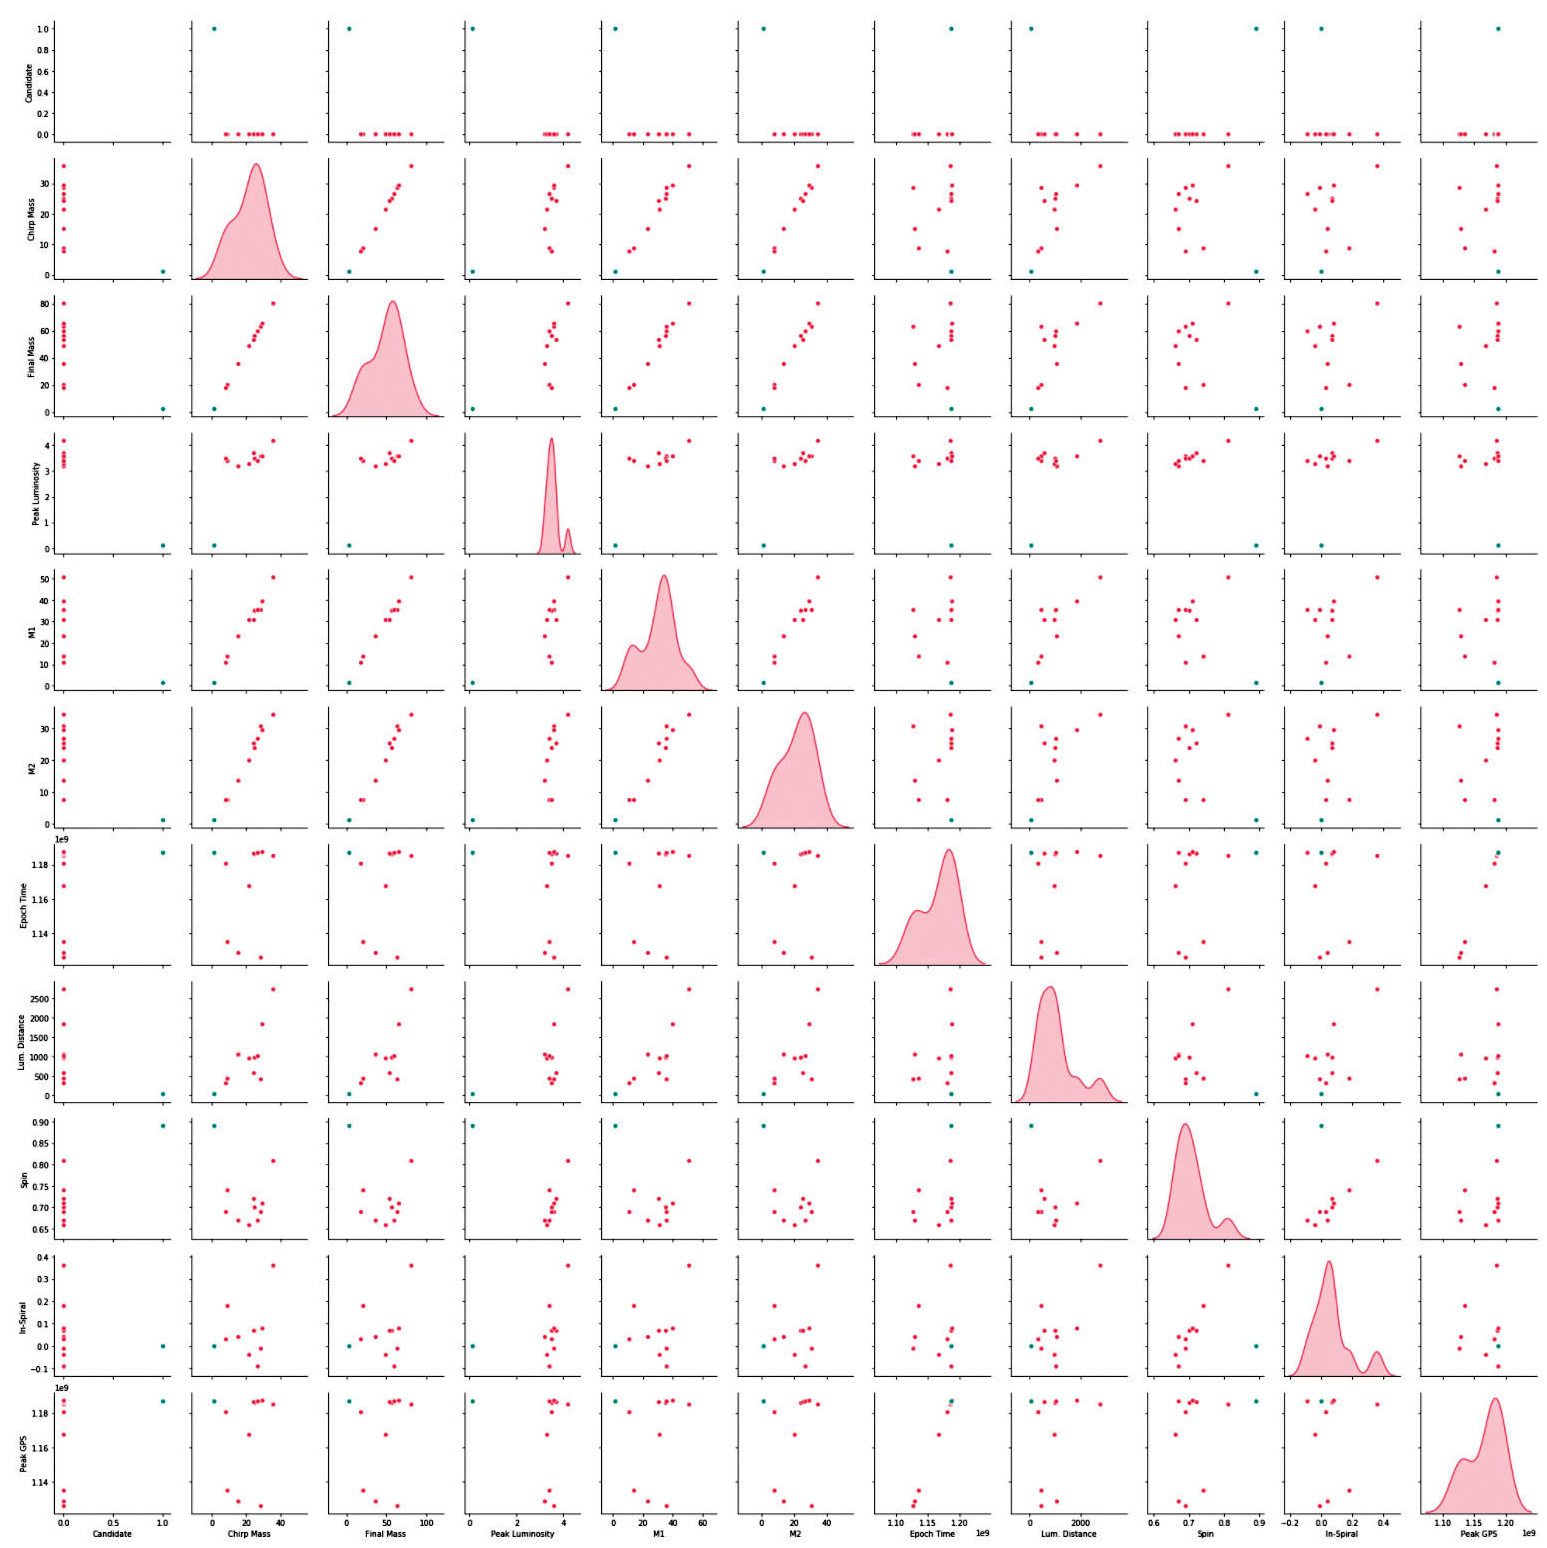
\includegraphics[width=1.0\linewidth]{images/52_09_Seconday-Data-Analysis_OmniView.jpg}
        \caption{\textit{Omni-view Plot of Secondary-Data-Analysis}}
        \label{fig:LIGO6_PlaceHolder_fig}
    \end{figure}

    This allows for the graphical comparison of any two parameters thereby helping us identify exceptional properties of various merger events and compare them to the standard ones as done in case of the 4 merger events ( GW170729, GW170817, GW190521 \& GW190814) selected using this exercise. Now by removing the leading diagonal and all repeated  in graphical plots he omni-plot shown in the above diagram, one can easily cluster dependent and independent variable clusters for building R-K models. A more detailed and usable version of this omni-plot is available on \url{https://dev.topobot.ai/}

    \subsubsection{Event Dendograms}

    The we have built an ontology of from the LIGO data based on dependent and independent variables pertaining to the various intrinsic physical parameters of the compact binary mergers which describes the hierarchic relationships between all physical measures to be taken into consideration for building the respective R-K models. The various selected attributes obtained using posterior probabilities and Bayesian parameter estimates are grouped as follows:
   
   \begin{itemize}
   	\item Primary Mass $(M_1)$, Secondary Mass $(M_2)$,Total Mass $(M_\odot)$, Chirp Mass $(M_\odot)$, Detector Frame Chirp Mass $(M_\odot)$ and Final Mass $(M_\odot)$ are all grouped together under the mass cluster which is dimensionally independent of all other clusters in the Dendogram. 
   	\item Similarly, all spin measures pertaining to $\chi_eff $ , In-spiral \& Final Spin get grouped together in the dimensionally independent spin cluster
   	\item We also consider 2 separate dimensionless ratios representing measures of Red-shift \& Q-values (ratio of Primary Mass $(M_1)$ \& Secondary Mass $(M_2)$,) in 2 separate independent clusters for comparing characteristic differences between Black Holes, Neutron Stars \& candidate Primordial Black Holes.
   \end{itemize}  
   
   it is important to note that it is not essential to pre-select a limited set of parameters from the source data (LIGO or otherwise) for the hierarchical feature extraction and building Dendograms using the R-K pipeline. We have chosen a subset of these specific parameters for the sake of simplicity and clarity in the first version of our implementation with reference to the latest developments in the filed of Gravitational Wave Astronomy.
   
   \begin{figure}[H]
   	\centering
   	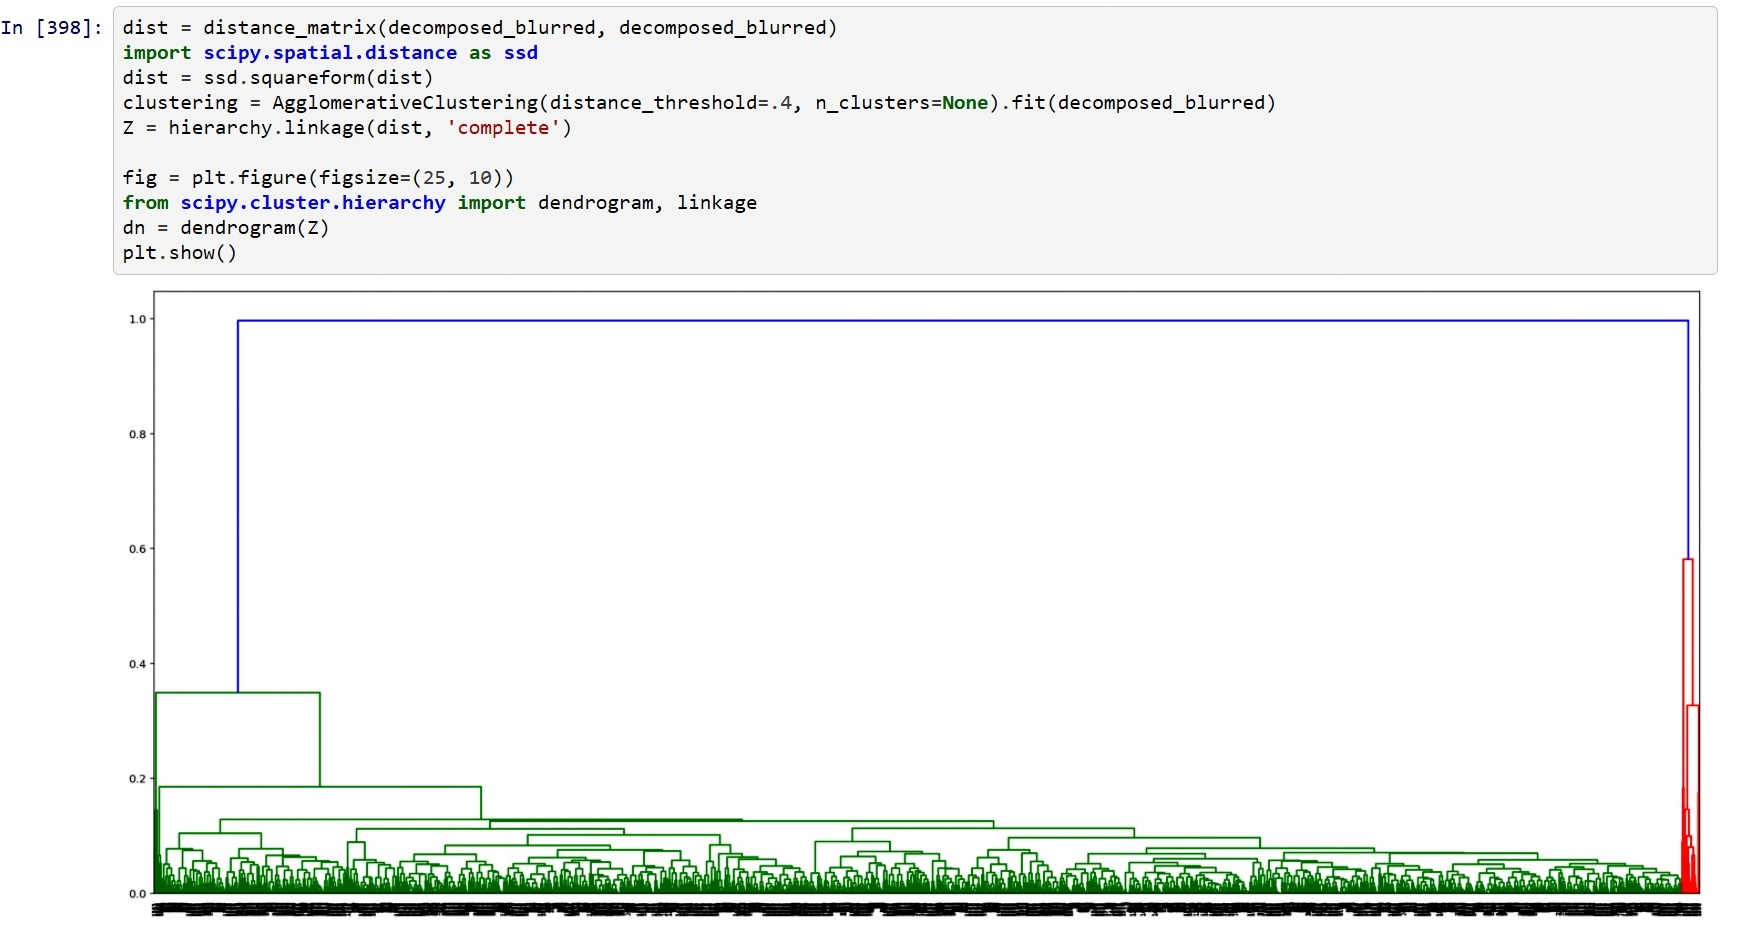
\includegraphics[width=1.0\linewidth]{images/56_12_Dendograms for Event Based Custering.jpg}
   	\caption{\textit{Dendograms for Event-Based Topological Clustering }}
   	\label{fig:LIGO7_PlaceHolder_fig}
   \end{figure}
   
   The above diagram shows the primary event node marked in 'red'. This serves as the event node to which the entire mass cluster has been linked via Hierarchical Feature Extraction techniques clustering all the  various mass attributes, i.e. Primary Mass $(M_1)$, Secondary Mass $(M_2)$,Total Mass $(M_\odot)$, Chirp Mass $(M_\odot)$, Detector Frame Chirp Mass $(M_\odot)$ and Final Mass $(M_\odot)$ grouped together in terms of their interdependencies as shown in the diagram.
   
    \subsubsection{Clustering of Bayesian Parameters}
    
In this section, we will address the hierarchy defined within each cluster with the example of the spin cluster as shown in the diagrams below. We shall also consider a single event GW 170729 for the purpose of demonstrating each step in this process. The R-K pipeline allows for the flexibility to scale and run clustering on all merger events in parallel resulting in the fundamental structural graph for Gravitational Wave Analysis based on LIGO data.  


    \begin{figure}[H]
        \centering
        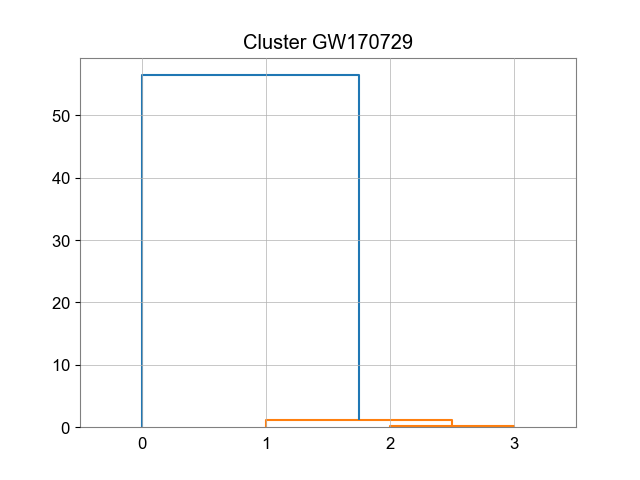
\includegraphics[width=1.0\linewidth]{images/57_13_GW170729 Event Based Dendogram.png}
        \caption{\textit{Single Event Dendogram GW170729}}
        \label{fig:LIGO8_PlaceHolder_fig}
    \end{figure}

The diagram above addresses the very first step of associated with a single event Dendogram. In this case the parent node or the 'event node' of the binary-merger event GW170729 first gets linked to one cluster at a time. In this case the diagram shows the linking of the spin cluster. All steps in this process take place in the Topological Phase Space and are independent of any choice of coordinates thereby ensuring scalability and flexibility of this framework.

    \begin{figure}[H]
        \centering
        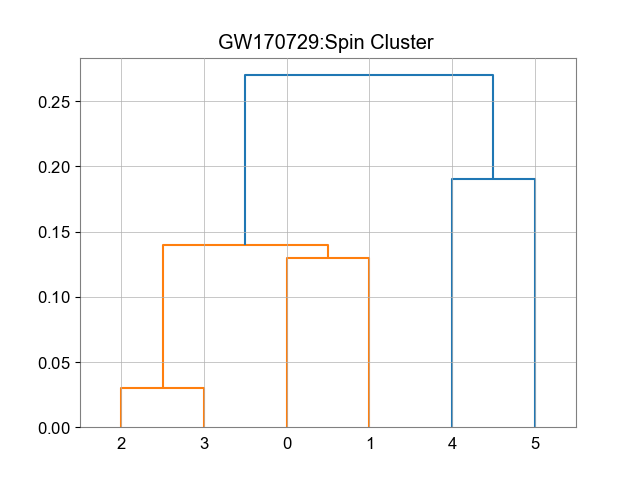
\includegraphics[width=1.0\linewidth]{images/61_17_GW170729 Spin Cluster.png}
        \caption{\textit{Spin Clustering of GW170729}}
        \label{fig:LIGO9_PlaceHolder_fig}
    \end{figure}

Now, we address the hierarchical grouping and ontological relationships within each cluster. The 3 measures of effective spin, in-spiral and final spin are ontologically linked and clustered together in an optimal way as shown in the figure above.

    \begin{figure}[H]
        \centering
        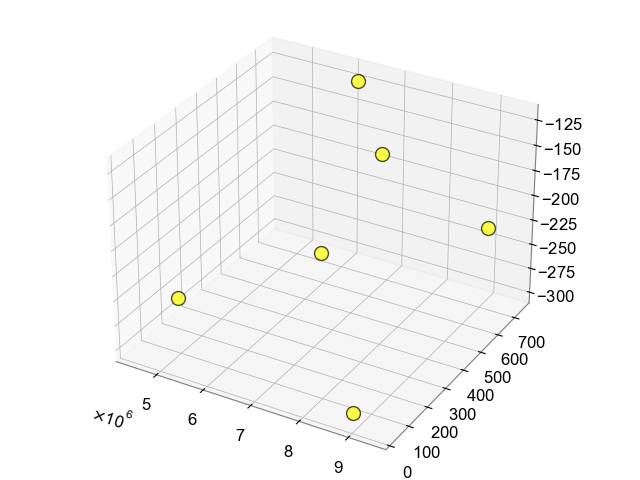
\includegraphics[width=1.0\linewidth]{images/65_21_Spin Nodes.png}
        \caption{\textit{Spin Nodes of 170729}}
        \label{fig:LIGO10_PlaceHolder_fig}
    \end{figure}
The next stage addresses all the nodes of each cluster separately in Phase Space. In this case it takes into account all values of each spin measure within the entire range of estimation error as indicated in the GWTC. for example in case of GW170729 the $\chi_eff = 0.37 $ with an error range of +0.21 to -0.25. Hence all min-max error range values are encoded into nodes along with the most probable  $\chi_eff = 0.37 $. 
    \begin{figure}[H]
        \centering
        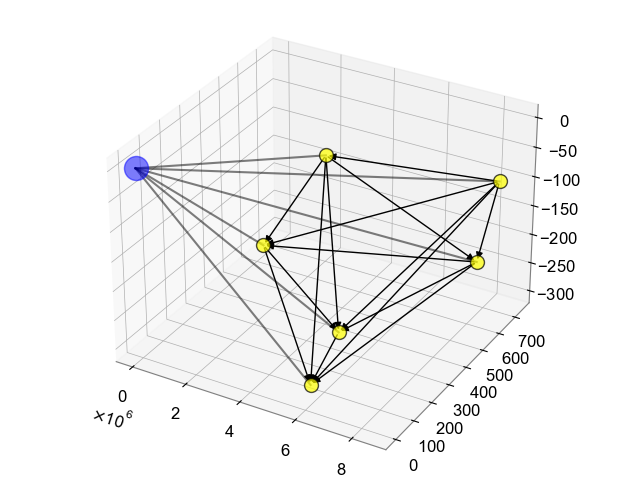
\includegraphics[width=1.0\linewidth]{images/Spin_Simplex3.png}
        \caption{\textit{Spin Simplex of 170729 linking with Central CBC Merger Event node marked in blue}}
        \label{fig:LIGO11_PlaceHolder_fig}
    \end{figure}

The final step links all the nodes in the correct manner directed to the highest or lowest value according to the choice of the user. However, in this case we have used the Leaf Linker to connect all the node values with edges within the cluster pointing towards the highest value of each measure. The edges also represent the entire range of possible values with any amount of granularity between the maximum and minimum range of each probable measure. This also gives rise to DAGs and simplicial complexes within each independent cluster of an R-K model. As a final step all nodes in each cluster are then linked to the parent node or the "event node" represented in blue in the above diagram. We have also carried out isometric-compression of such structural graphs based on the euclidean distance using the Leaf Linker algorithm. This single linkage clustering was also done via the Leaf Linker available as a part of the R-K toolkit.

\subsubsection{Unfiltered Structural Graphs}


The steps described in the above section were carried out in parallel on each of the selected binary-merger events. This gave rise to 4 independent structural graphs for the binary merger events:  GW170729, GW170817, GW190521 \& GW190814, as shown in the diagram below.

    \begin{figure}[H]
        \centering
        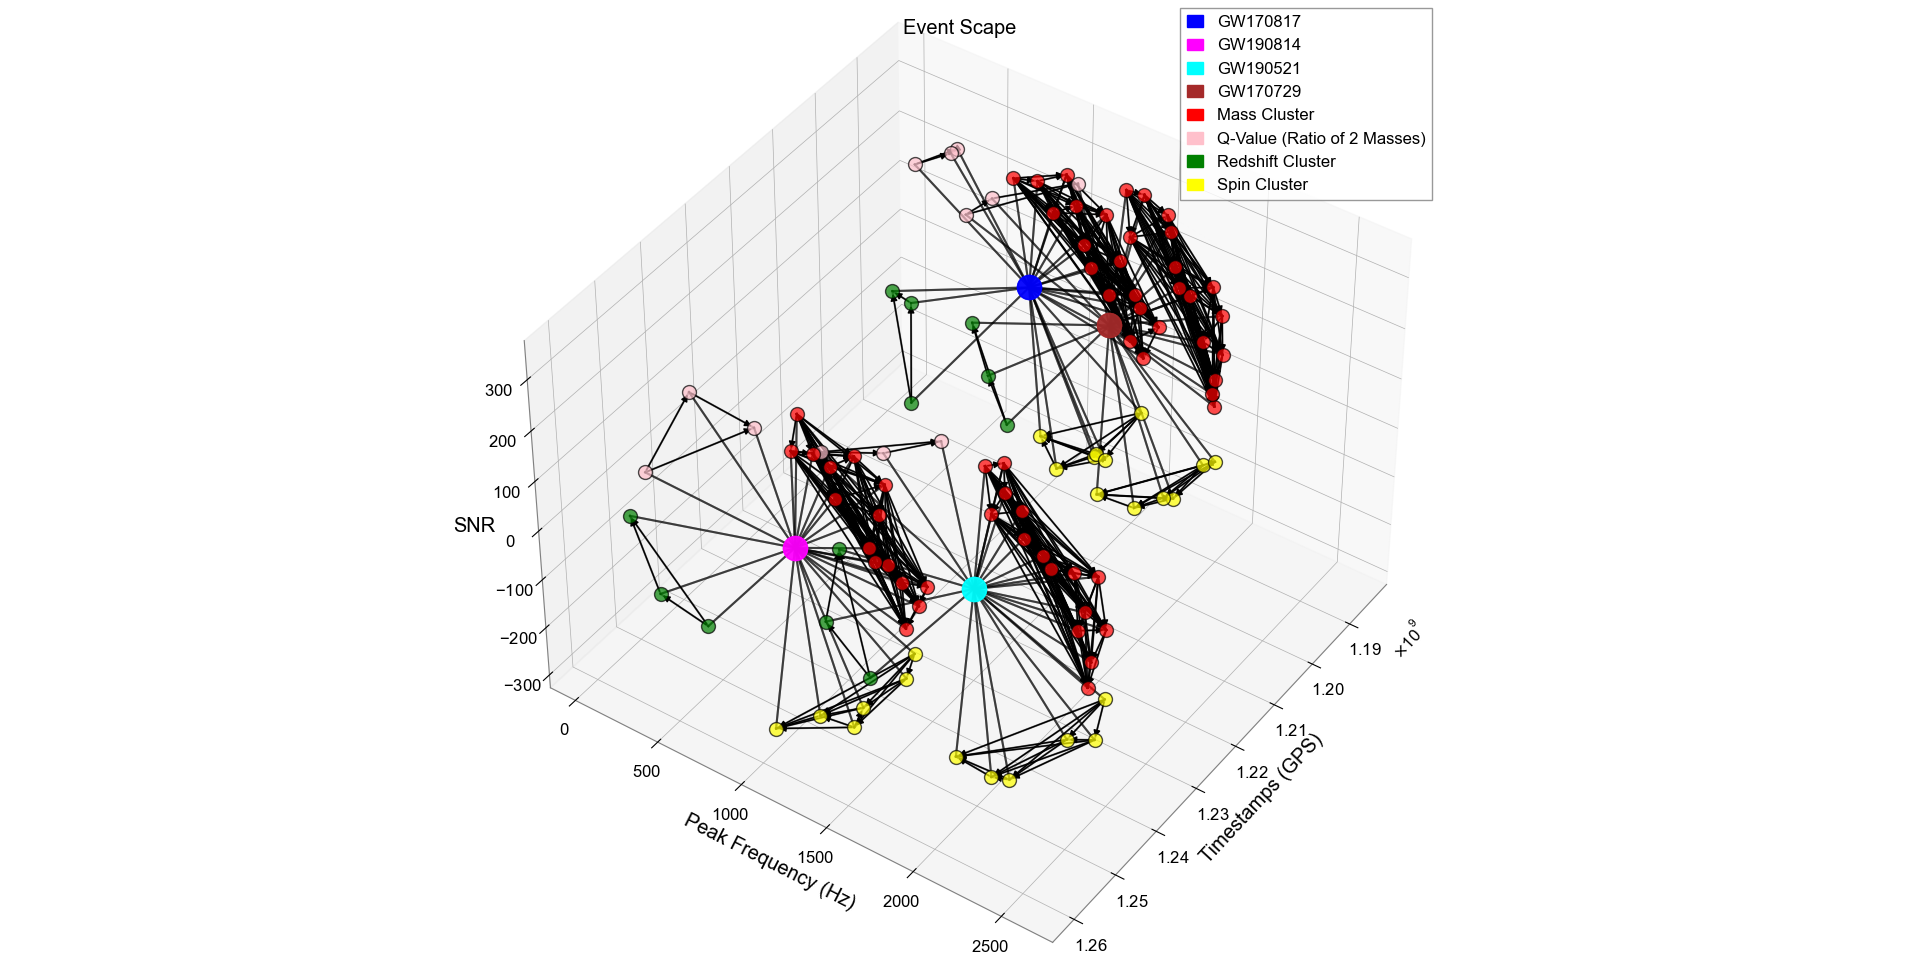
\includegraphics[width=1.0\linewidth]{images/70_26_EventScape of 4 RK Diagrams without Threshold Filters 2.png}
        \caption{\textit{Event-scape of 4  Unfiltered Structural Topologies with linked multi-graphs as generated by the R-K Pipeline}}
        \label{fig:LIGO12_PlaceHolder_fig}
    \end{figure}
However, as detailed in the previous case-study with store-sales data, these structural graphs rise purely out of all data-points available in the columns of the high-dimensional dataset. Thus node masks and filter functions need to be applied to obtain unique event-driven R-K Diagrams as discussed in section \ref{sec:Filters} .

\subsubsection{Data Filters \& Sensitivity Thresholds}

The modified R-K pipeline for LIGO comes with a built-in visualizer and a GUI to track each step of the process from loading primary/raw strain data all the way up to plotting R-K diagrams. This is given to users to enable the smooth application of node masks and range filters to all the selected clusters of unfiltered R-K models for all binary merger events. One can use the GUI to run through and validate each step of the process described in this case study. 

    \begin{figure}[H]
        \centering
        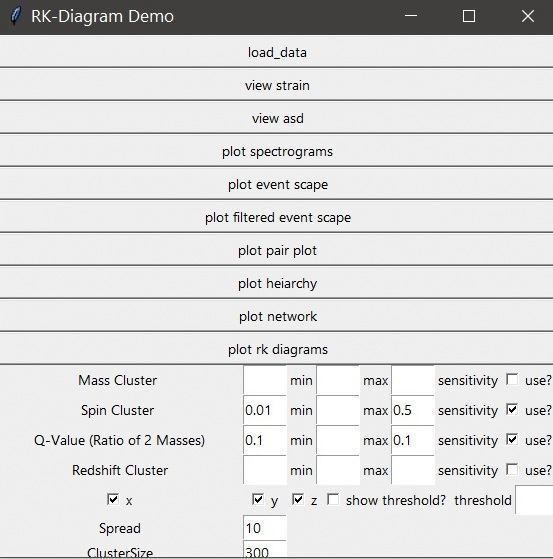
\includegraphics[width=1.0\linewidth]{images/71_00_Sensitivity Thresholds.jpg}
        \caption{\textit{Sensitivity Thresholds and domain specific filters applied to the R-K Pipeline }}
        \label{fig:LIGO13_PlaceHolder_fig}
    \end{figure}

Hence the GUI in the above diagram allows parameter based topological filtering of the base structural graph or the R-K model in a way such that node masks and range filters either suppress or express components of each independent cluster based on any chosen measure and its corresponding filter parameters. In this case our objective was to find R-K diagrams with all spin measures close to 0 and low q-value ratios of around 0.1 in order to segregate potential neutron-star mergers from stellar black holes and primordial black holes. The mass cluster values add further distinction in terms of determining whether the compact binaries are in the mass gap. The choice of these parameters were driven by well established research in this field. \cite{00.7_LIGOBayesianAnalysis} \cite{00.6_LIGOAnalysisPipeline} \cite{24.5_GWParameterEsitmation} \cite{24.7_qvalueestimation} \cite{24.8_PBHdetectionparameters} \cite{24.9_EffectiveSpin}

\subsubsection{Final R-K Diagrams}
    
    
Thus Parameter Based Topological Filtering was carried out on selected clusters such as Mass, Spin, Q-Ratio \& Red-shift with the Range Filter algorithms applied within pre-set ranges of $\chi_eff=0.01$ \&  $q=0.1$  \cite{24.7_qvalueestimation} \cite{24.9_EffectiveSpin} \cite{00.6_LIGOAnalysisPipeline}considering all error bars to obtain the corresponding R-K diagrams of the 4 selected events as described blow in the order of their GPS merger times.

    \begin{figure}[H]
        \centering
        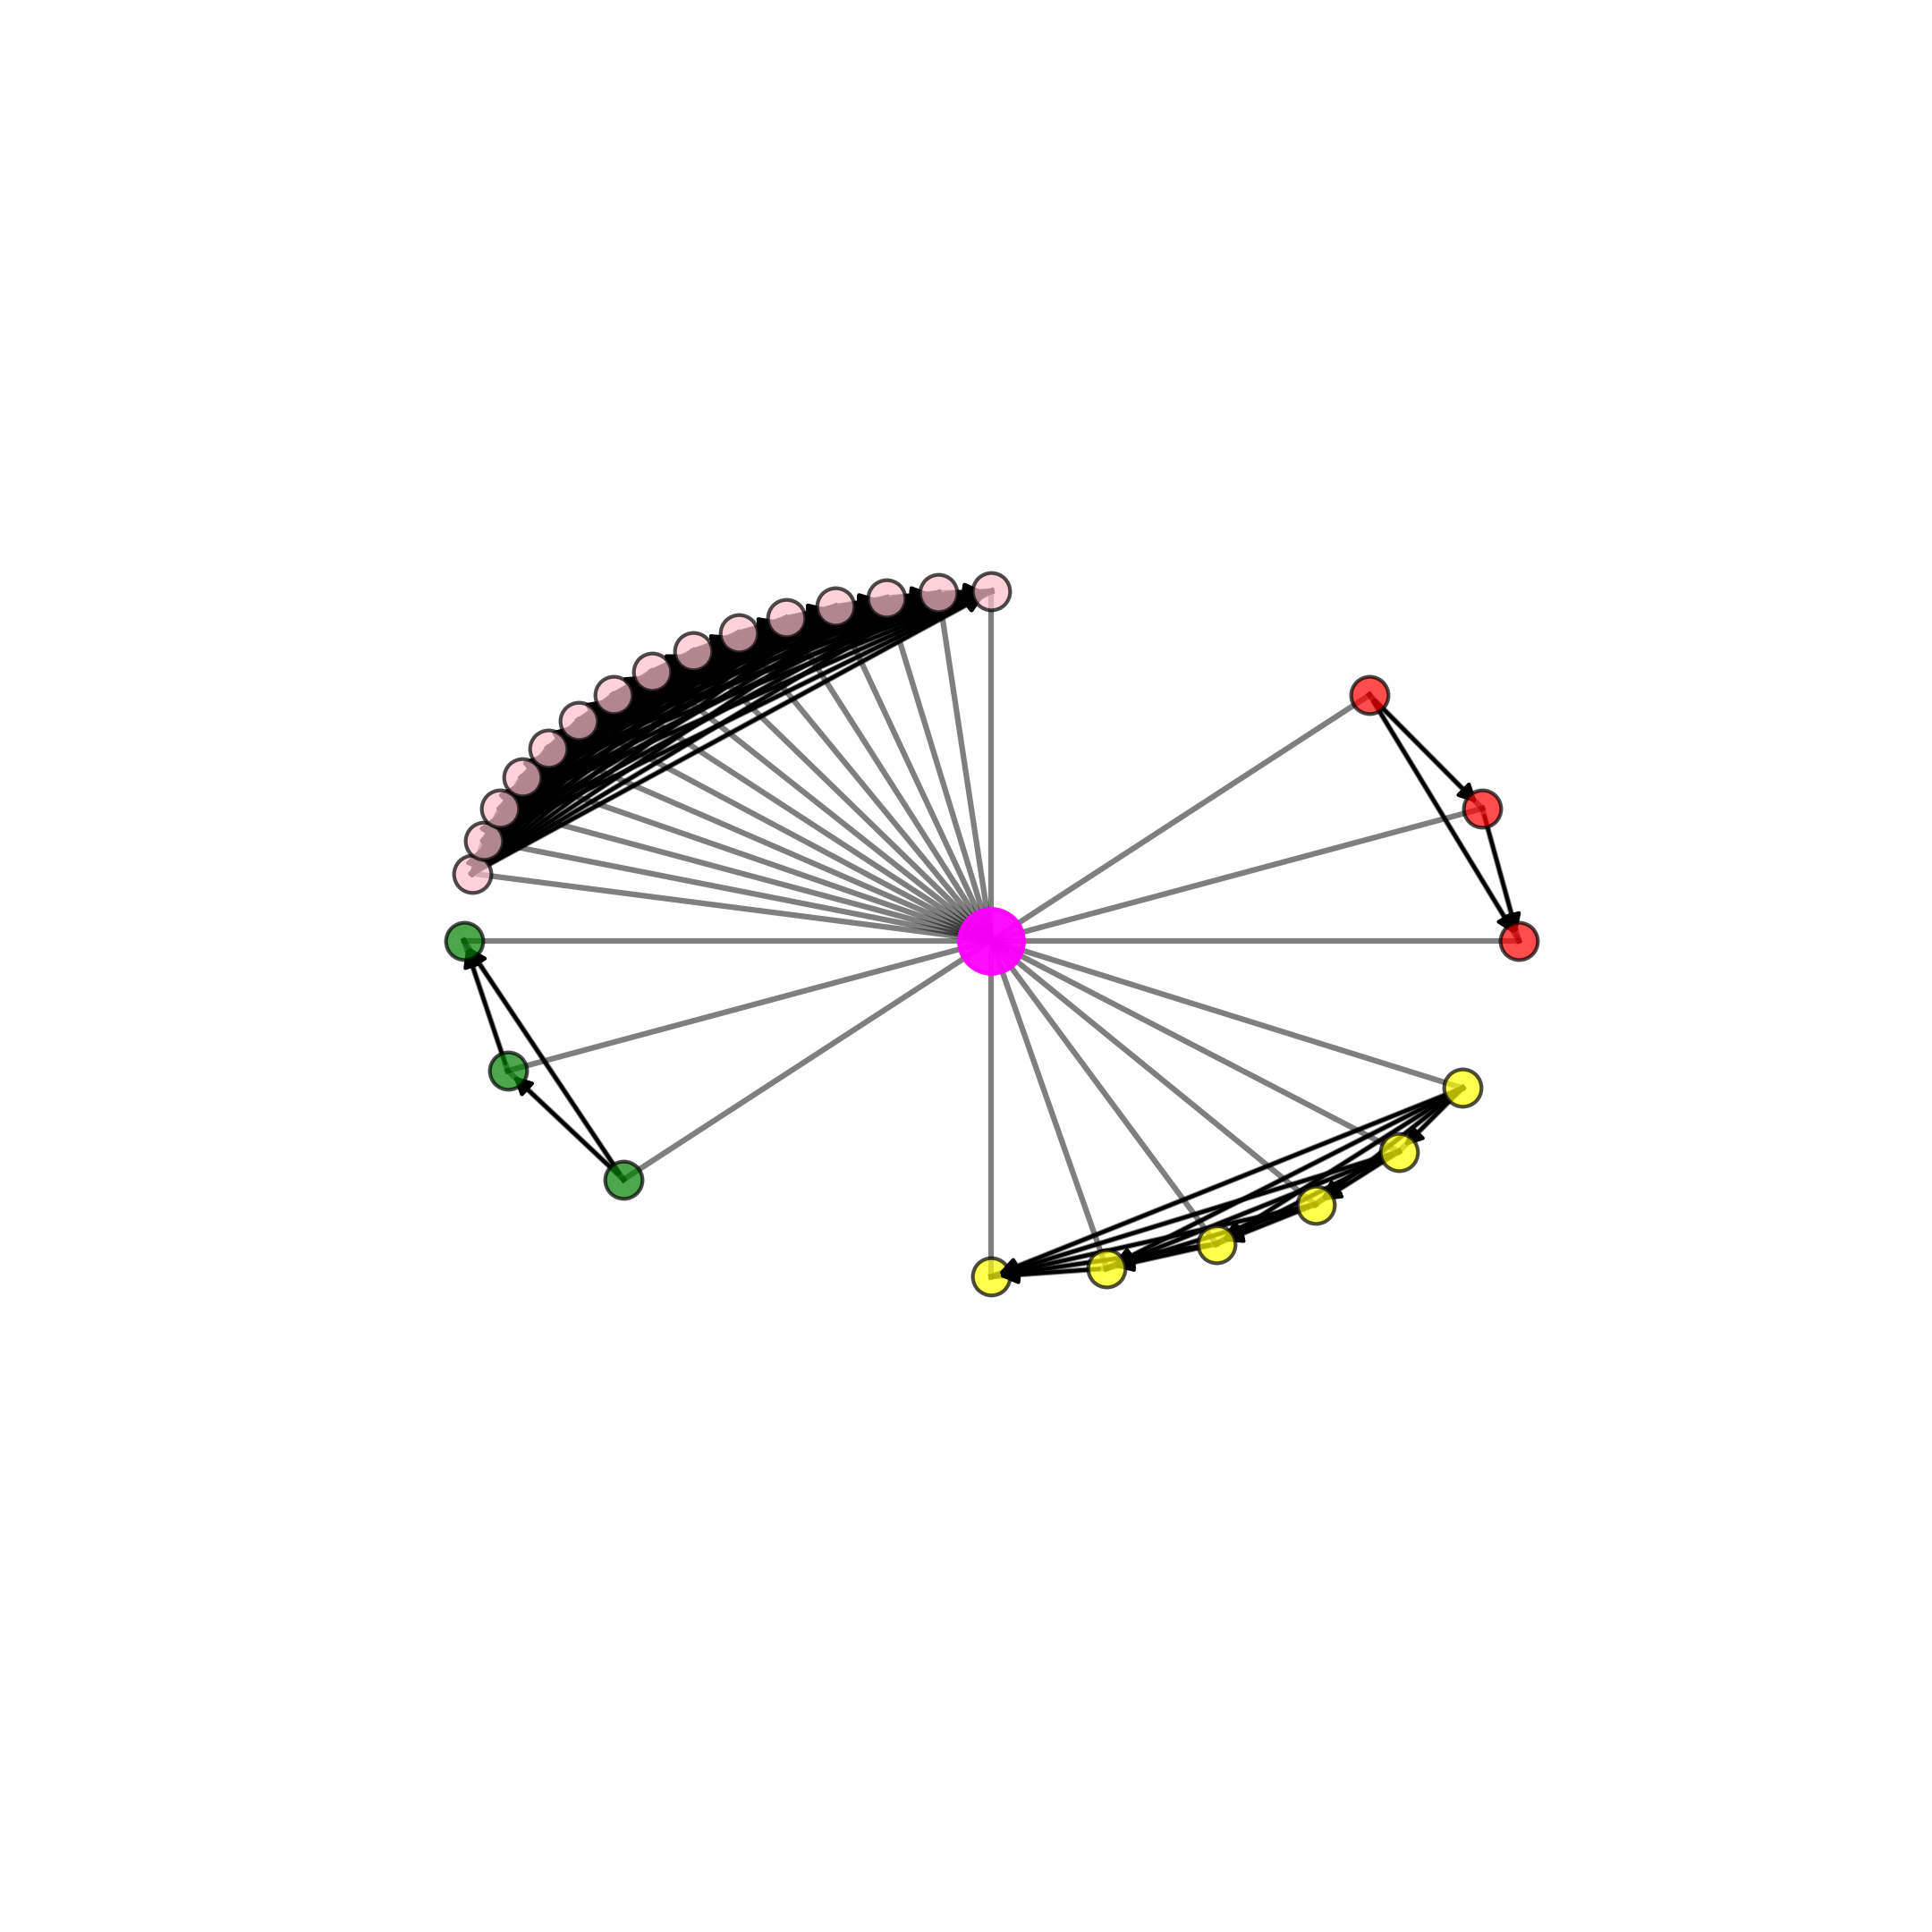
\includegraphics[width=1.0\linewidth]{images/GW170729_RK_Diagram.png}
        \caption{\textit{Final R-K Diagram of GW170729}}
        \label{fig:LIGO14_PlaceHolder1_fig}
    \end{figure}

The first R-K Diagram under consideration is that of the event GW170729 as shown above. In this case we find $\chi_eff \le 0.058$ \&  $q\ge 1.09$. The mass values don't fall in the mass gap range and hence represent all characteristics of a typical stellar black hole.

    \begin{figure}[H]
        \centering
        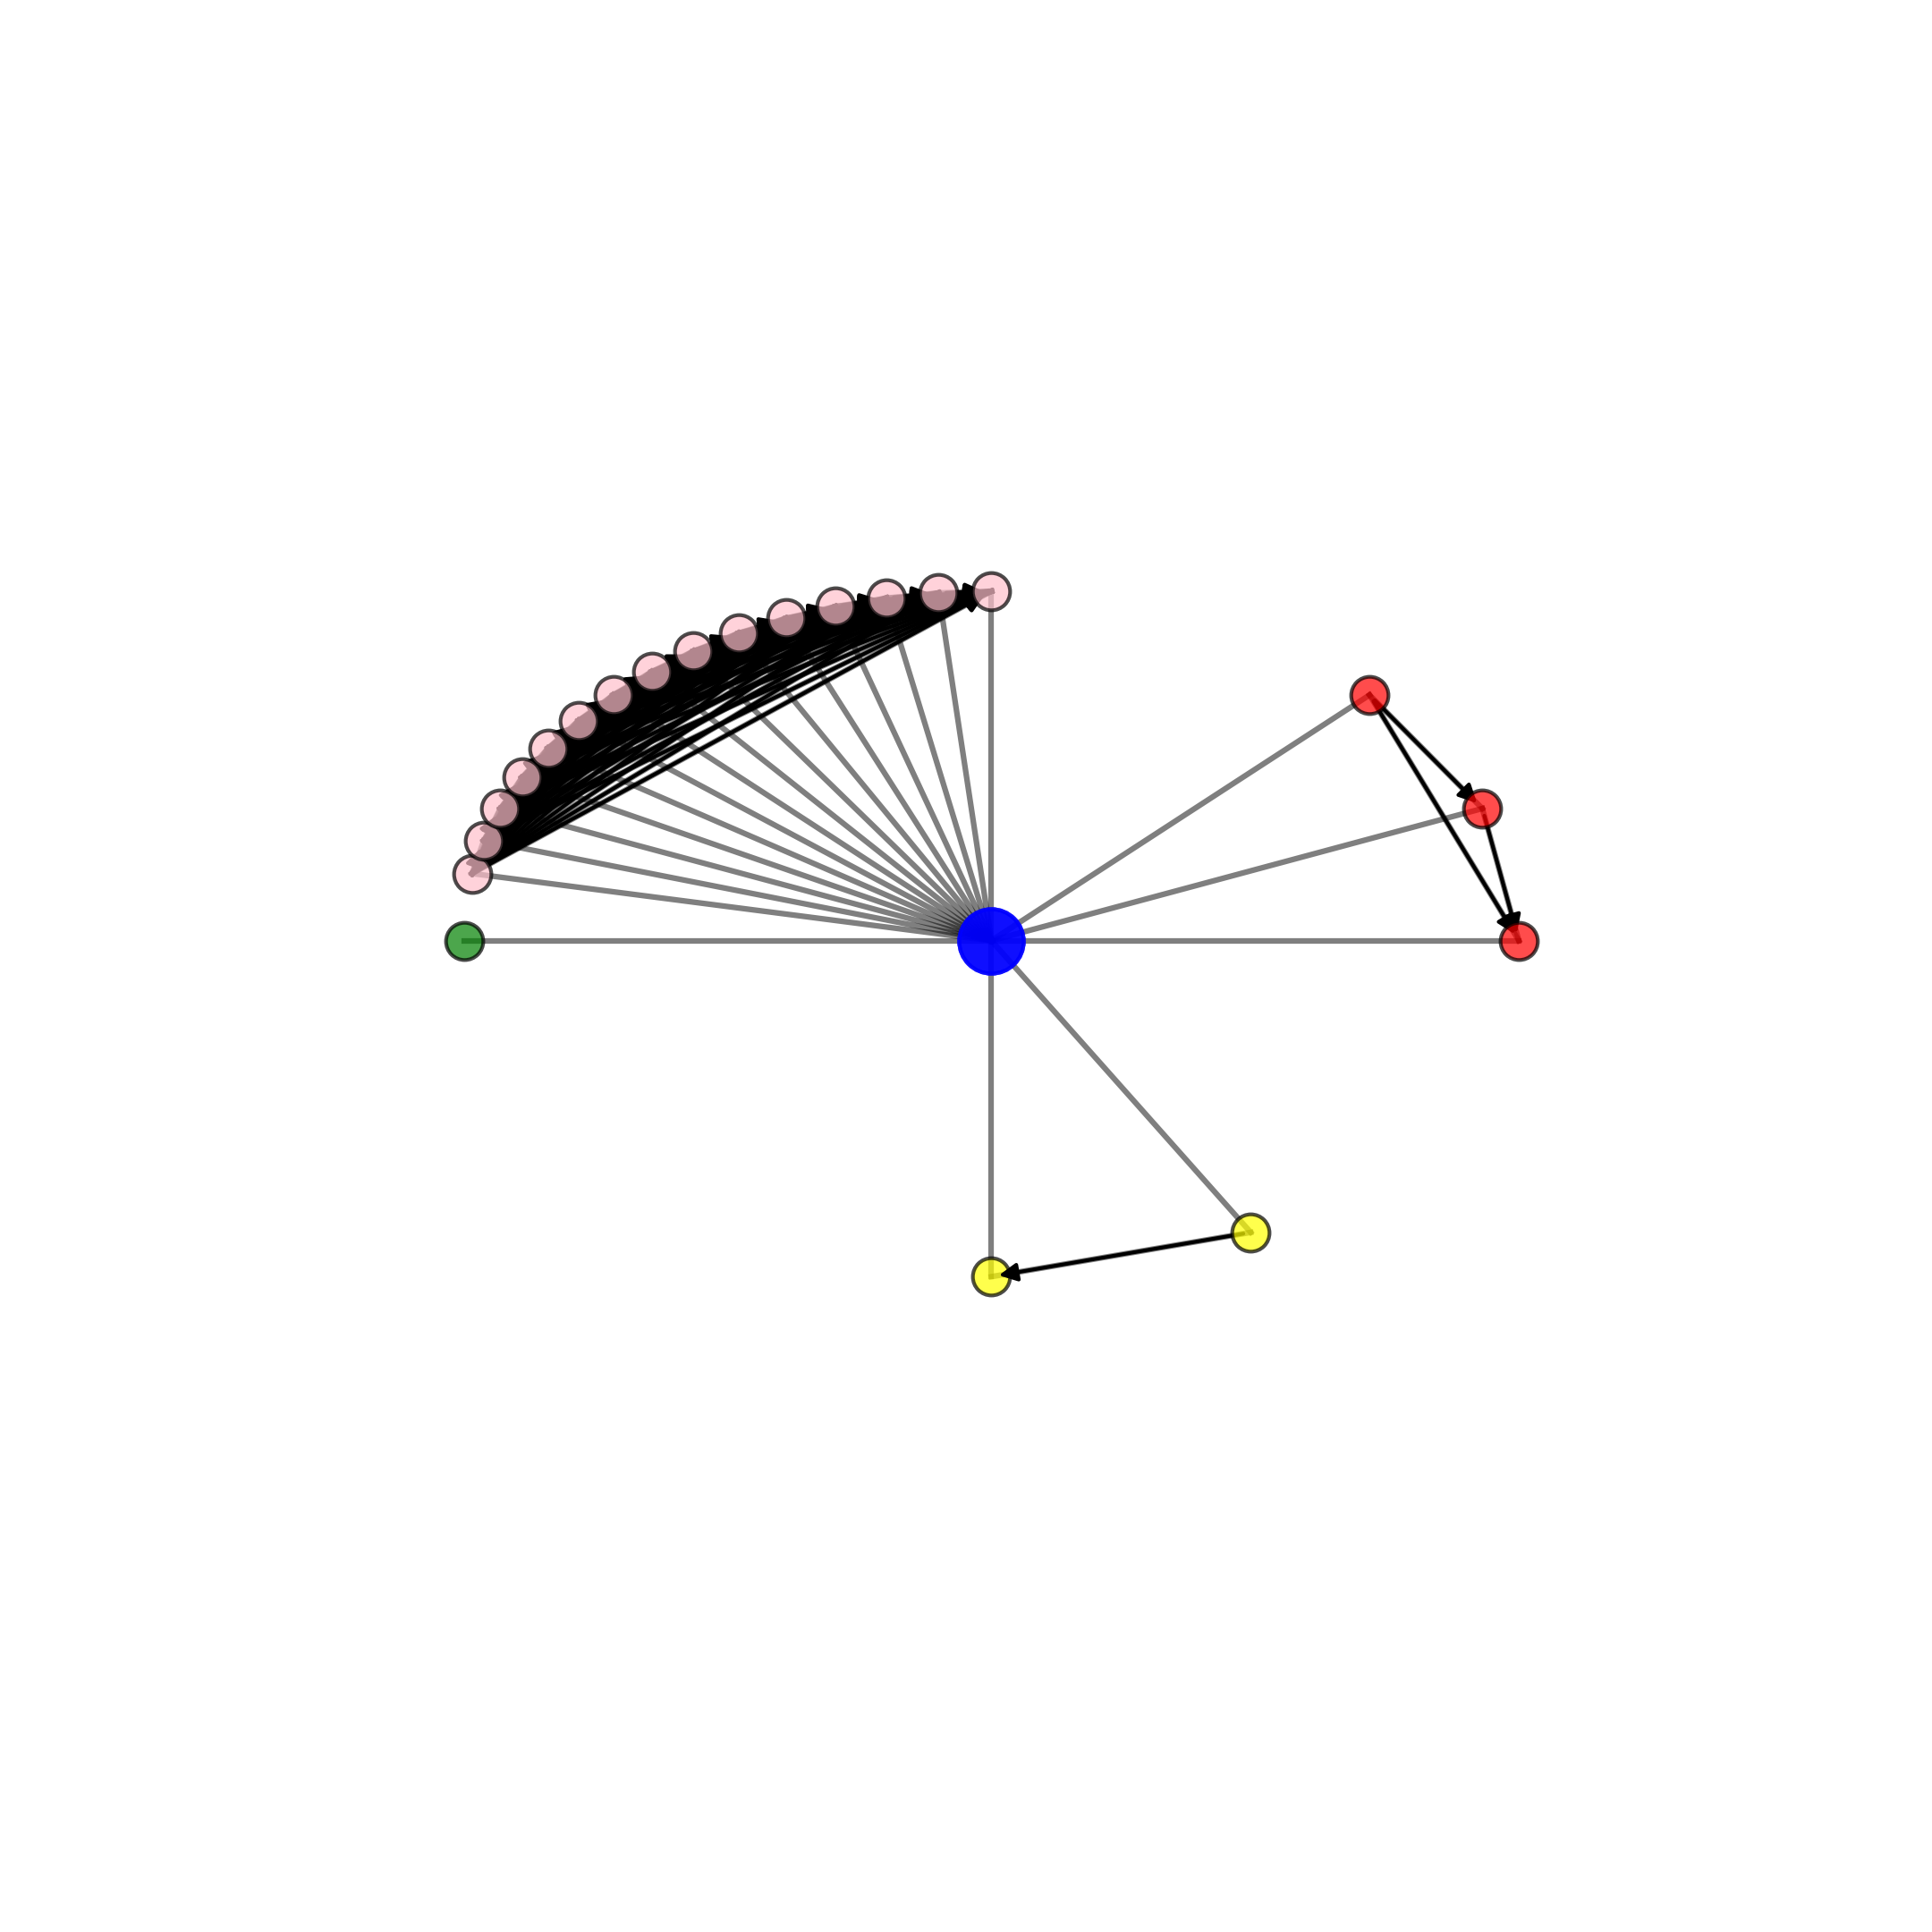
\includegraphics[width=1.0\linewidth]{images/GW170817_RK_Diagram.png}
        \caption{\textit{Final R-K Diagram of GW170817}}
        \label{fig:LIGO14_PlaceHolder2_fig}
    \end{figure}

The second R-K Diagram under consideration is that of the event GW170817 as shown above. In this case we find $\chi_eff = 0.01$ \&  $q\le 0.89$. The mass values don't fall in the mass gap range but the q value differs significantly from that of a candidate primordial black hole. This can be further verified by adding an electromagnetic counter-part from multi-messenger data which has been left out of scope for the purpose of this paper but could be easily added to the R-K models by extending the R-K pipeline in future. Thus the detection of an electromagnetic counterpart, with low $\chi_eff$ close to 0 and q value close to 1 establishes this event as a compact binary NS-NS (Neutron Star) merger.

    \begin{figure}[H]
        \centering
        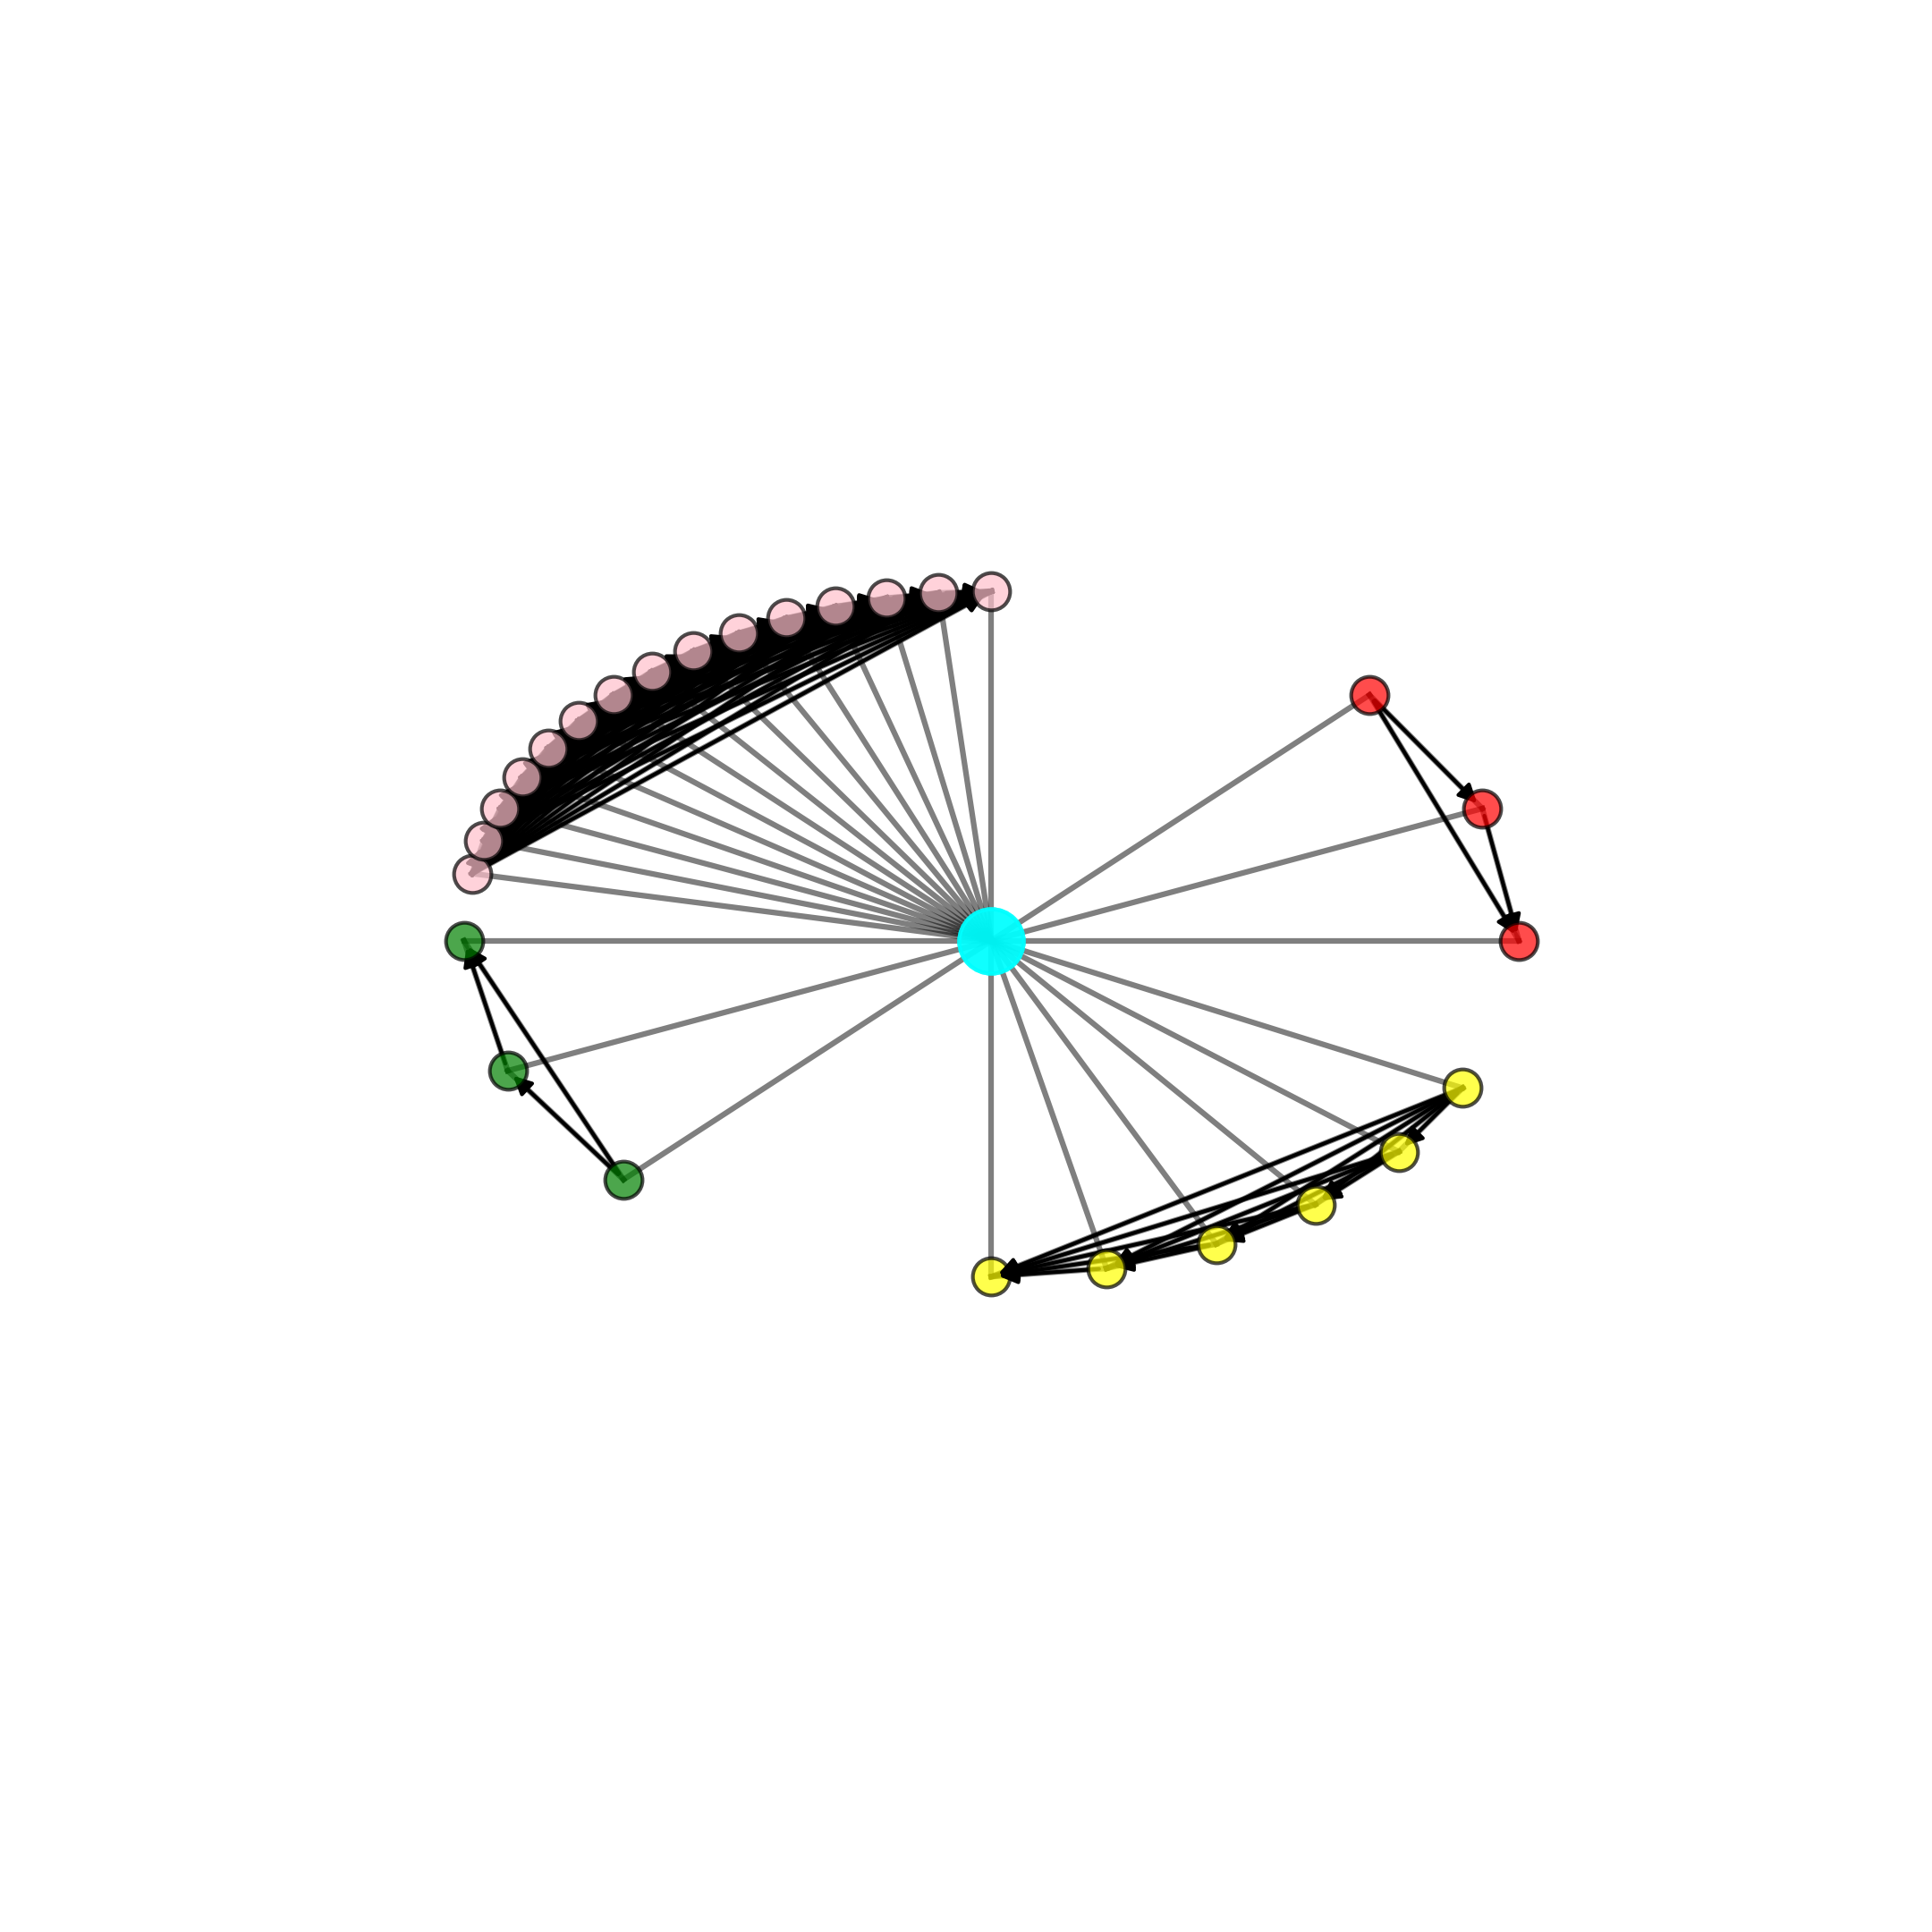
\includegraphics[width=1.0\linewidth]{images/GW190521_RK_Diagram.png}
        \caption{\textit{Final R-K Diagram of GW190521}}
        \label{fig:LIGO14_PlaceHolder3_fig}
    \end{figure}

The third R-K Diagram under consideration is that of the event GW190521 as shown above. In this case we find $\chi_eff \le 0.9$ \&  $q\ge 4$. The mass values don't fall in the mass gap range and hence this binary merger event also represents all characteristics of a typical stellar black hole much like GW170729 and both have topologically similar R-K diagrams.

    \begin{figure}[H]
        \centering
        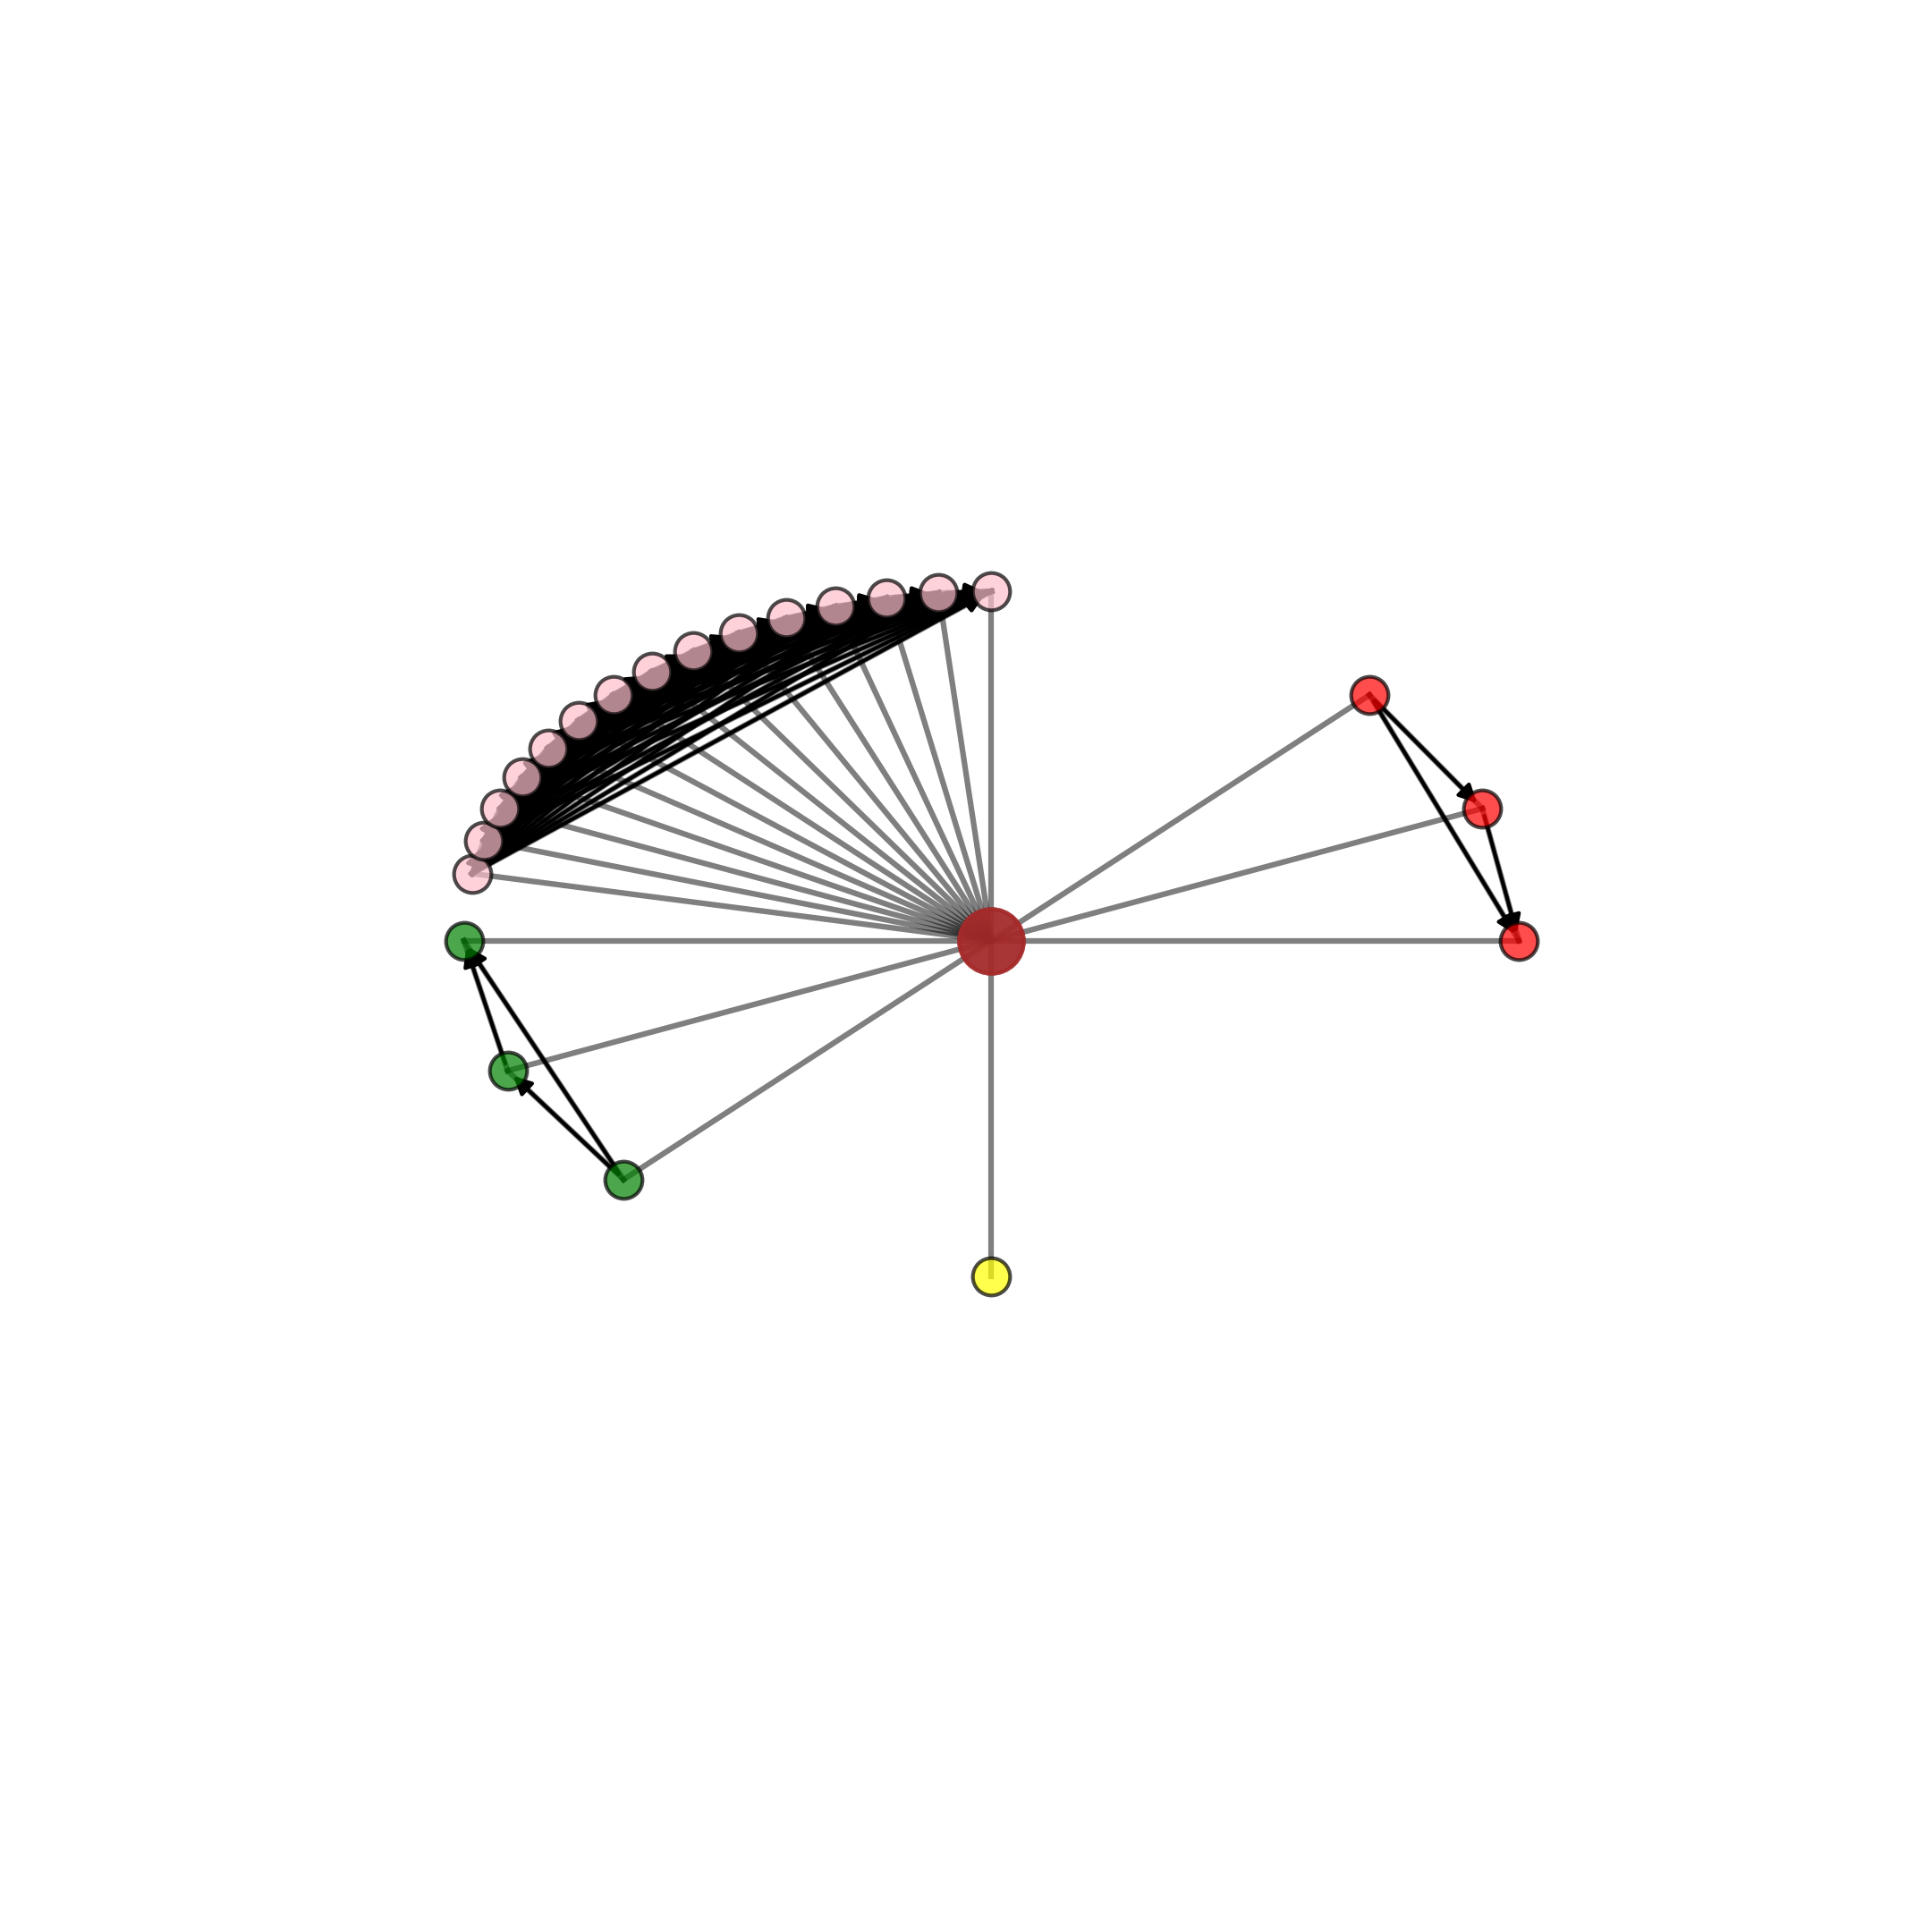
\includegraphics[width=1.0\linewidth]{images/GW190814_RK_Diagram.png}
        \caption{\textit{Final R-K Diagram of GW190814}}
        \label{fig:LIGO14_PlaceHolder_fig}
    \end{figure}

The fourth and final R-K Diagram under consideration is that of the event GW190814 as shown above. This is also the most interesting one under consideration as in this case we find $0.04 \le \chi_eff \le 0.05$ \&  $q = 0.1$. The mass values  definitely fall in the mass gap with no electromagnetic counterpart. Hence it has a lot of prominent features that are indicative of a candidate Primordial Black Hole (Dark Matter). However, further increase in detector sensitivity combined with added parameters such as more accurate detection of high Red-shifts which would be a distinguishing characteristic of candidate Primordial Black Holes. However, LIGO and VIRGO are currently not sensitive enough to detect such high red-shifts and therefore we require more sensitive probes like the Einstein Telescope for further parameter based distinction in future. But as discussed earlier, the R-K pipeline is designed in a highly scalable manner to include Multi-messenger data-streams in future to provide further distinction between R-K diagrams of different compact binary mergers.  

\subsubsection{Untuned R-K Diagram Event-Scape}

Thus all R-K diagrams of any given set of compact binary merges can be represented in a transformed Event-scape in 3D space with the x-axis representing the GPS time, y-axis representing the peak frequency values and the z axis representing the amount of SNR or signal to noise ratio as shown in the diagram below. The higher the SNR value the more confident we can be with respect to the detection and classification of distinct compact binaries.

    \begin{figure}[H]
        \centering
        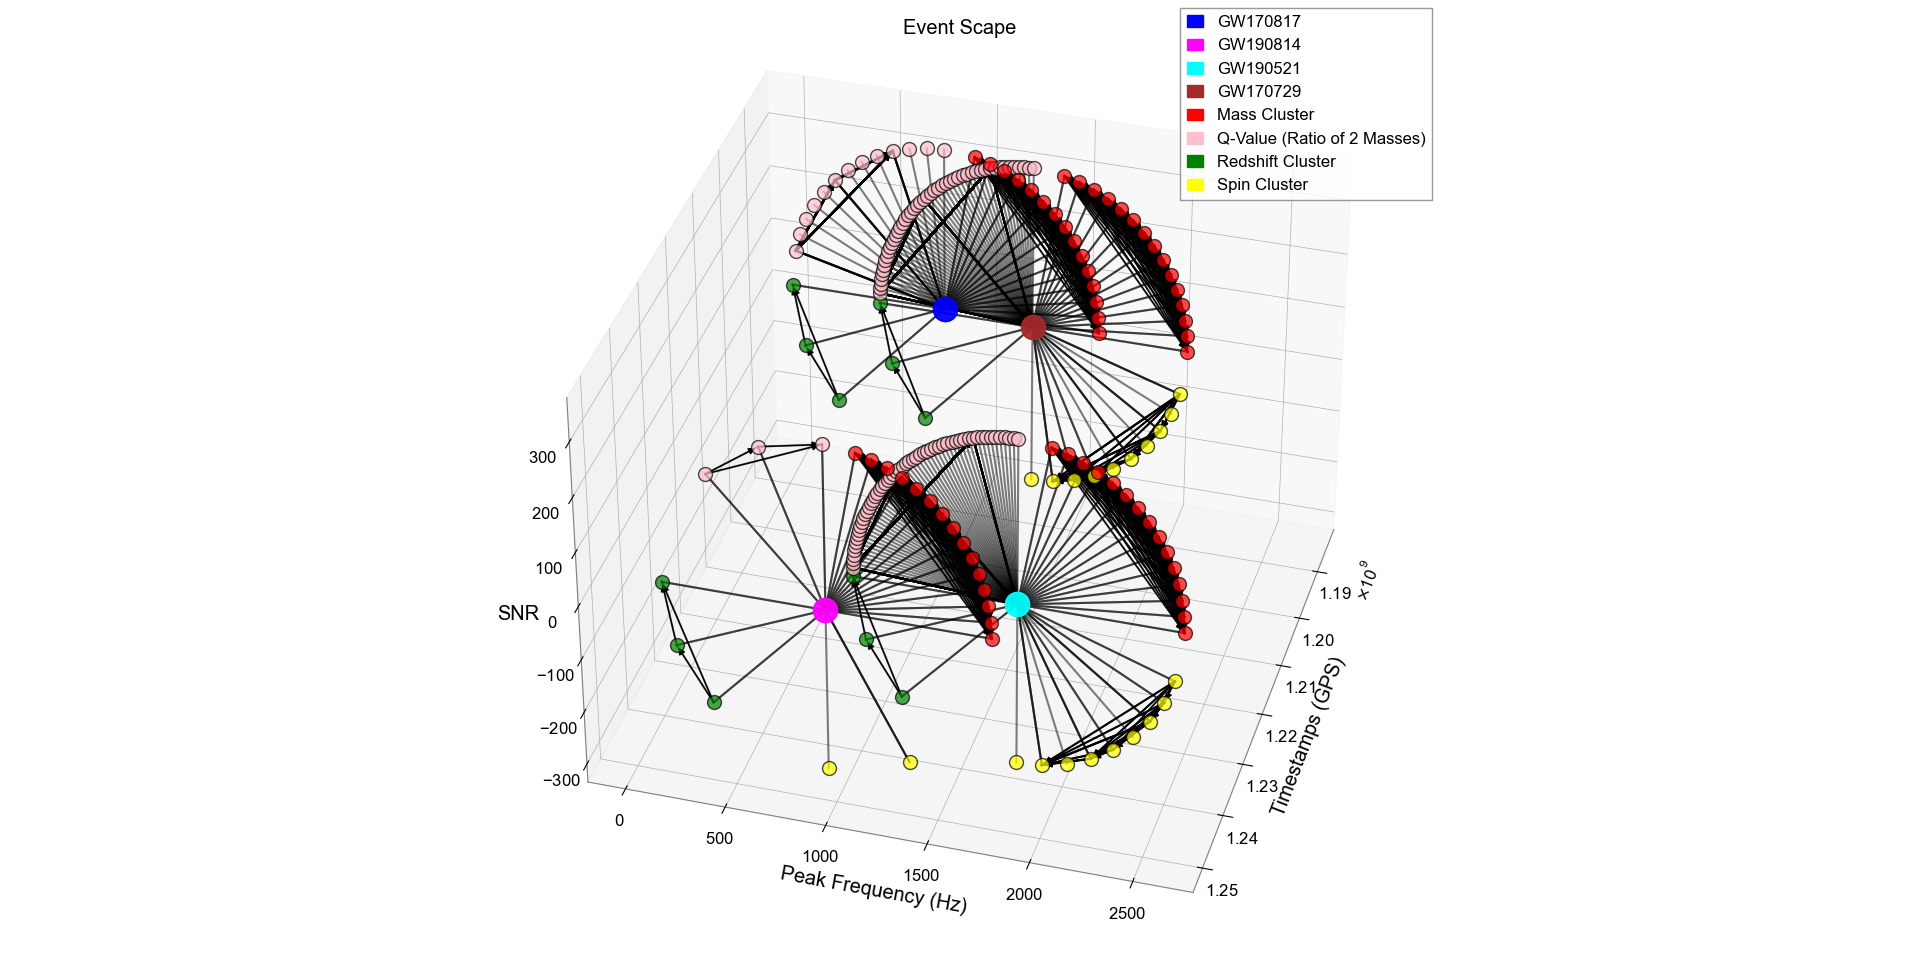
\includegraphics[width=1.0\linewidth]{images/74_33_All 4 Diagrmas in 3D_2.png}
        \caption{\textit{All 4 Event Based R-K Diagrams in 3D}}
        \label{fig:LIGO15_PlaceHolder_fig}
    \end{figure}

The above diagram shows multiple merger events plotted in the event-scape for which the topological distance or divergence and similarity measures were computed using templates from matched filters with respect to the 4 selected events. In order to test the accuracy and effectiveness of classification we set template labels on the 4 classified events. In order to show a proof of concept we assigned absolute labels to all 4 merger events such that GW170729 and GW190521 were assigned the label of BH-BH merger, GW170817 was labelled as a NS-NS merger and GW190814 was labelled as a PBH-PBH merger.

This resulted in an initial average intra-class topological distance separation of \textbf{0.17} between BH-BH mergers upon applying the parameter specific Range Filters and Node Masks discussed in the previous sections. This would imply an intra-class similarity of \textbf{0.83} between BH-BH mergers. It was also interesting to note an inter-class topological distance separation of \textbf{0.32} between BH-BH and confident NS-NS mergers which would imply a lower order inter-class similarity of \textbf{0.68} and verifies the effectiveness of R-K diagrams and the R-K pipeline to a significant extent. Comparative studies based on similarity measures of the candidate PBH was left for the next section as no clear or conclusive results were obtained using the untuned  models. 


\subsubsection{Tuned Results for Template based Classifications}

In order to maximize divergence across R-K Diagrams, we trained our models using Facebook's Nevergrad \cite{a2020_nevergrad} optimizers. Thus, as demonstrated in the below sections, by providing an objective function and iterating over the various R-K models in a stochastic batch, we were able to reduce total loss of the set across different labelled classes over 1000 iterations.

After optimization, we encoded the R-K Diagram into a vector and trained an SVM over the vectorized diagrams to produce a binary classifier over the data where X represents each vectorized R-K Diagram and Y are labels of PBH Merger events. Thus the pipeline required two levels of optimization. The SVM generated a plane of separation between R-K diagrams as shown in the form of a grid in the diagram below.

    \begin{figure}[H]
        \centering
 	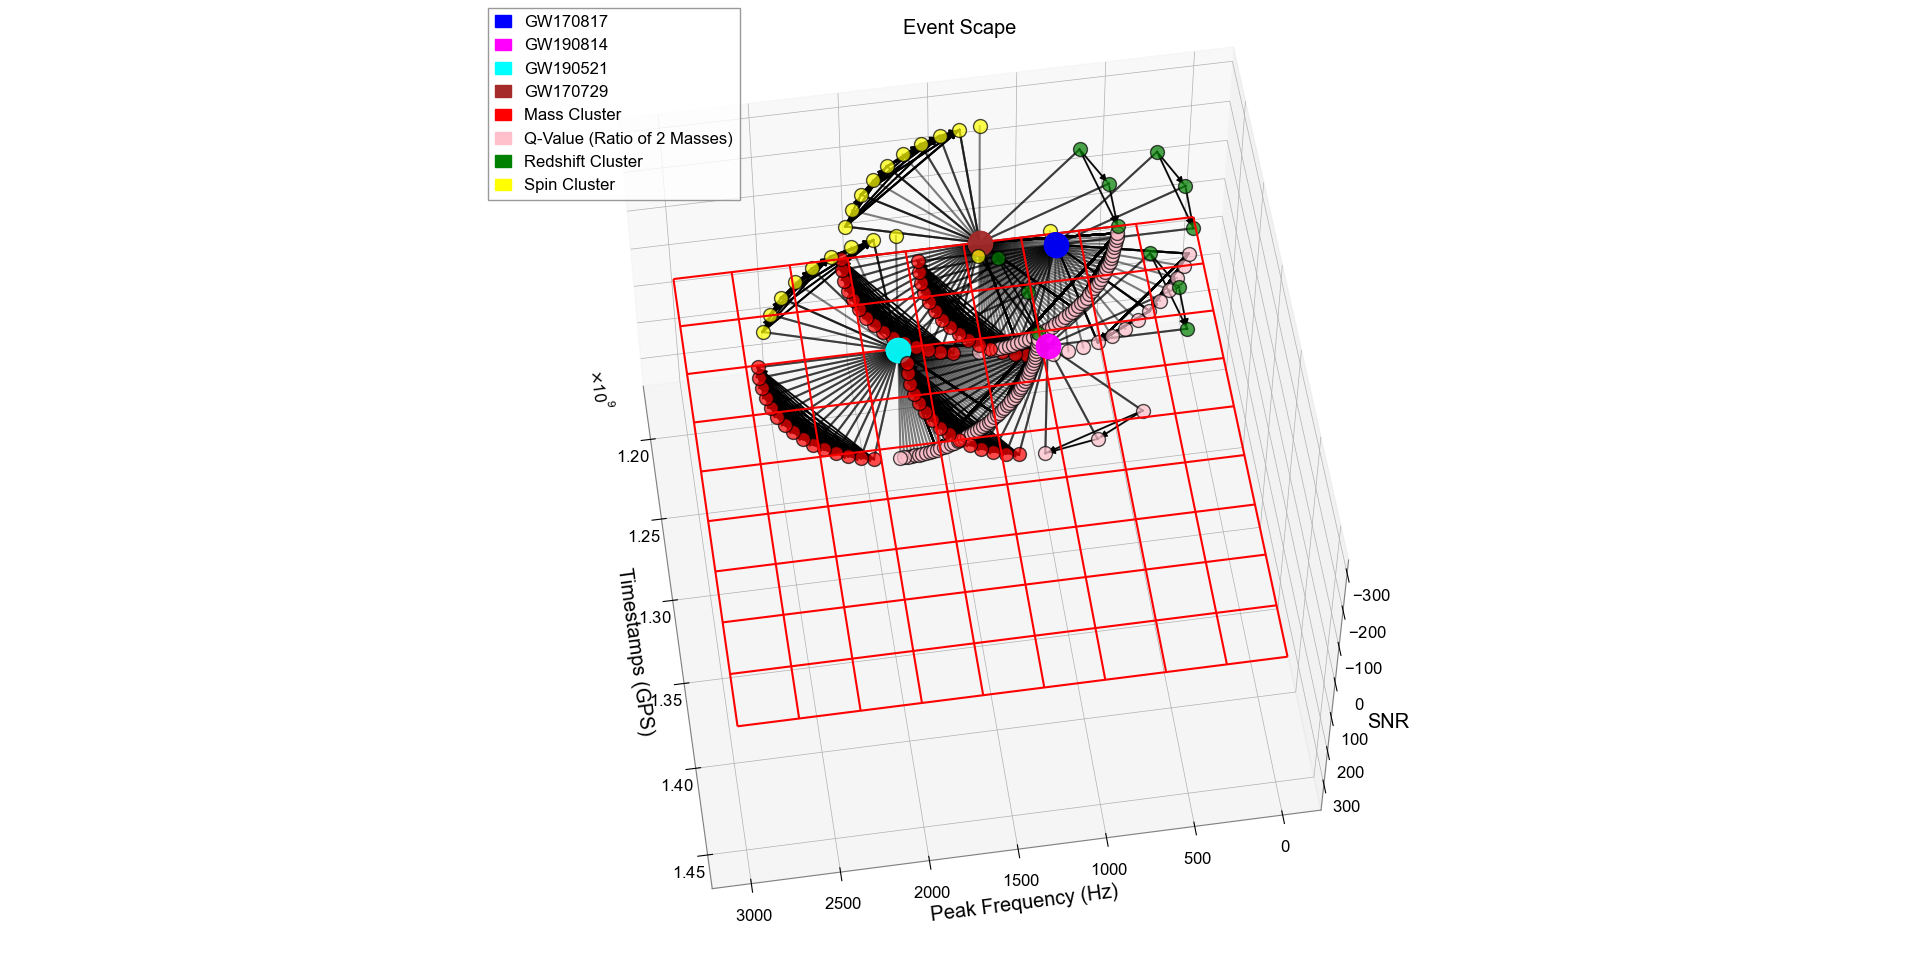
\includegraphics[width=1.0\linewidth]{images/75_34_All-4-Diagrmas-in-3D_with-SNR_3.png}
 	\caption{\textit{All 4 Event Based R-K Diagrams in 3D with SVM threshold grid}}
 	\label{fig:LIGO16_PlaceHolder_fig}
 \end{figure}

This gave us closer intra-class topological separation between BH-BH mergers which were recorded with an average similarity measure between the range of $\lbrack0.9, 0.96\rbrack$ and NS-NS Mergers between a range   $\lbrack0.59, 0.65\rbrack$. The candidate PBH measured an interclass similarity of 0.71 with w.r.t. to NS-NS mergers and 0.62 w.r.t. BH-BH mergers with distinctly different R-K Diagrams. However, a more detailed study of the unique topological signatures and R-K diagrams of Primordial Black Holes is definitely promising but beyond the scope of this paper and should be left for future research due to the lack of conclusive data and sufficient observational parameters at present.

\subsection{Localization of R-K Diagrams}

We localised the R-K Diagrams using the T--distributed Stochastic Neighbour Embedding (TSNE). T-SNE is a tool to visualize high-dimensional data by trying to minimize Kullbak-Leibler Divergence between low dimensional embeddings and the higher-dimensional data. \cite{sklearn.manifold.tsne_2014}. Using the original data, we localized to a two dimensional surface each root of the R-K Diagram by using summary information of the R-K model using metric and topological evaluation methods.

\begin{figure}[H]
	\centering
        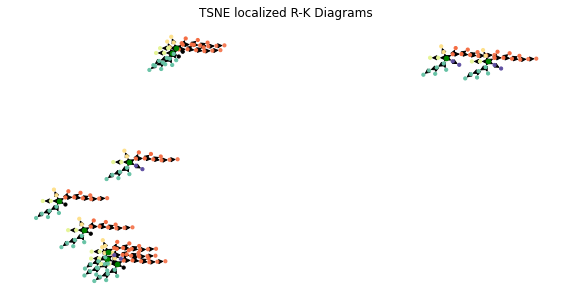
\includegraphics[width=0.5\textwidth]{images/TSNELocalizedRKDiagrams.png}
	\caption{\textit{TSNE localized R-K Diagrams}}
	\label{fig:tsne}
\end{figure}

\subsection{Multi-modal Classification of CBCs using R-K Diagrams}


\begin{figure}[H]
	\centering
	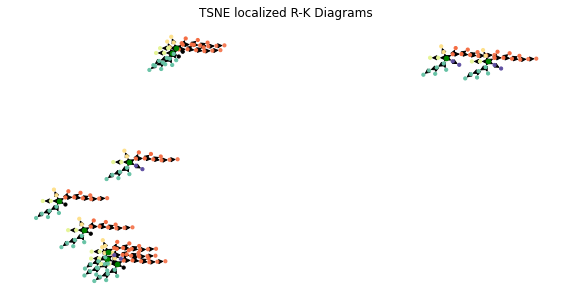
\includegraphics[width=0.5\textwidth]{images/TSNELocalizedRKDiagrams.png}
	\caption{\textit{TSNE localized R-K Diagrams}}
	\label{fig:tsne2}
\end{figure}

\subsubsection{R-K Event-Scape vs Primary Analysis}
 
 The fine-tuned results of the R-K Event-Scape provides distinct categorical R-K diagrams representing a specific class of compact binary mergers as shown in the previous section. However, it is important to note that these fine-tuned R-K diagrams can then be remapped to the Q-transformed spectral densities from Primary Analysis.  
 
 \begin{figure}[H]
 	\centering
 	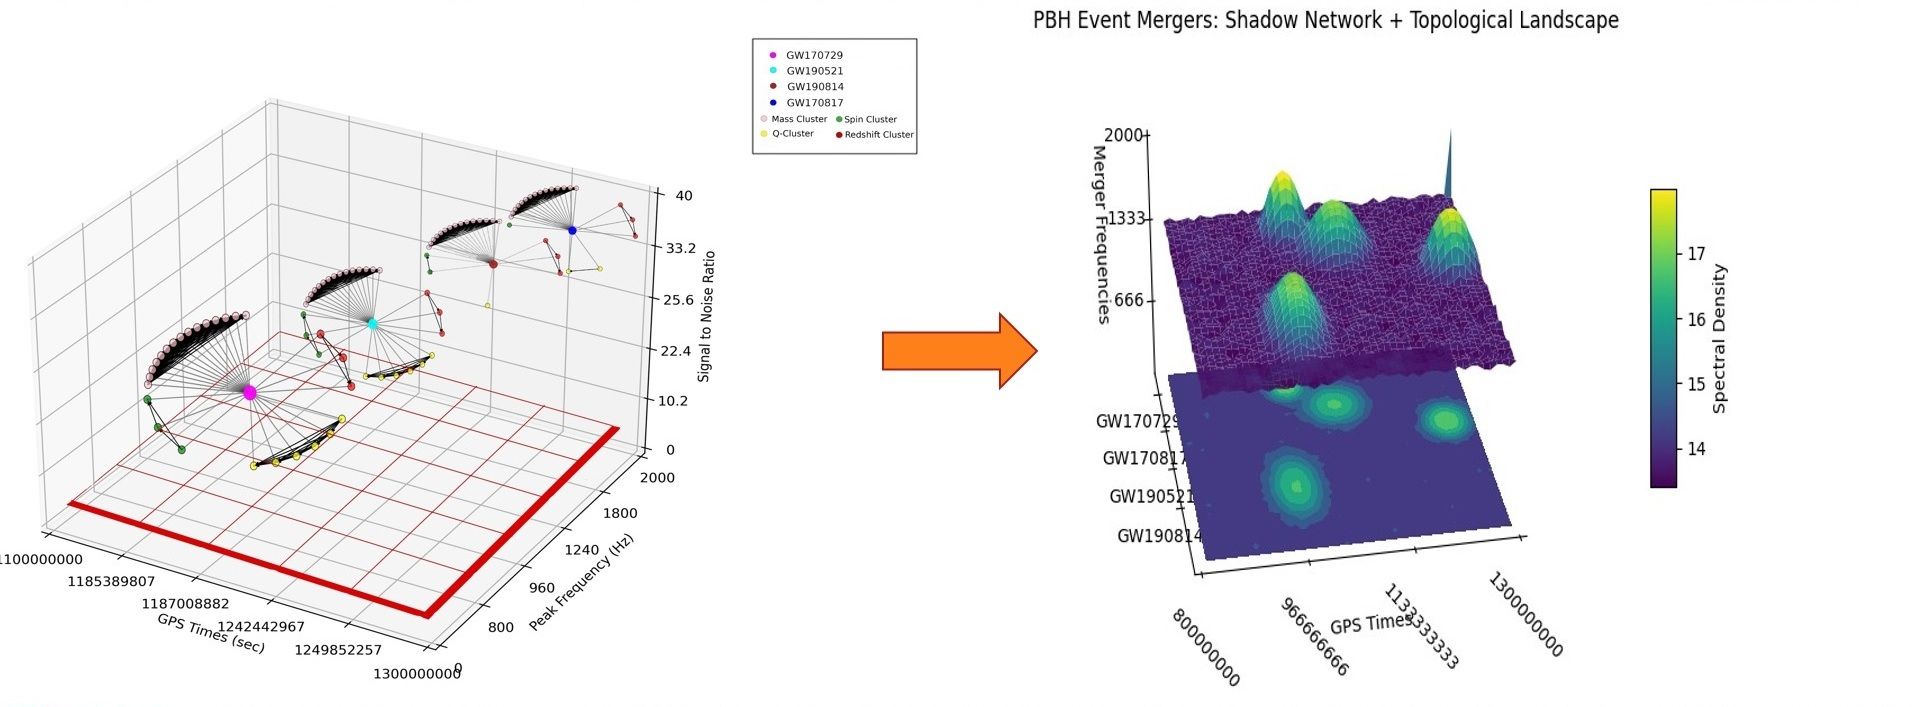
\includegraphics[width=1.0\linewidth]{images/76_Mapping R_K eventScape to Primary Data.jpg}
	\caption{\textit{Mapping R-K Event-Scape to Primary Data}}
 	\label{fig:LIGO17_PlaceHolder_fig}
 \end{figure}

A study could then be conducted using the automated R-K pipeline to find any meaningful correlations between the the topological characteristics of the merger signals obtained form the detectors at source and their corresponding labelled counterparts obtained in the form of R-K Diagrams from the R-K pipeline. Since the final R-K Diagrams have been vectorized for the purpose of classification using SVMs, therefore they could serve as templates for the segregation and classification of future gravitational wave merger signals  obtained from compact binary mergers after the established steps of noise-filtering are carried out on the same. This would allow for near-real time segregation and classification of confident binary mergers which would keep improving over time with the addition of more SVM parameters from Multi-messenger data-streams and future advancements in LIGO. 

 \subsection{Scope of Future Work}

In this section we have showcased an example of a schematic representation of how the R-K pipeline could complement and augment the capabilities of  the current LIGO Analysis Pipeline which has been published by Abbott et.al. \cite{00.6_LIGOAnalysisPipeline} as shown in the diagram below.

\begin{figure}[H]
	\centering
	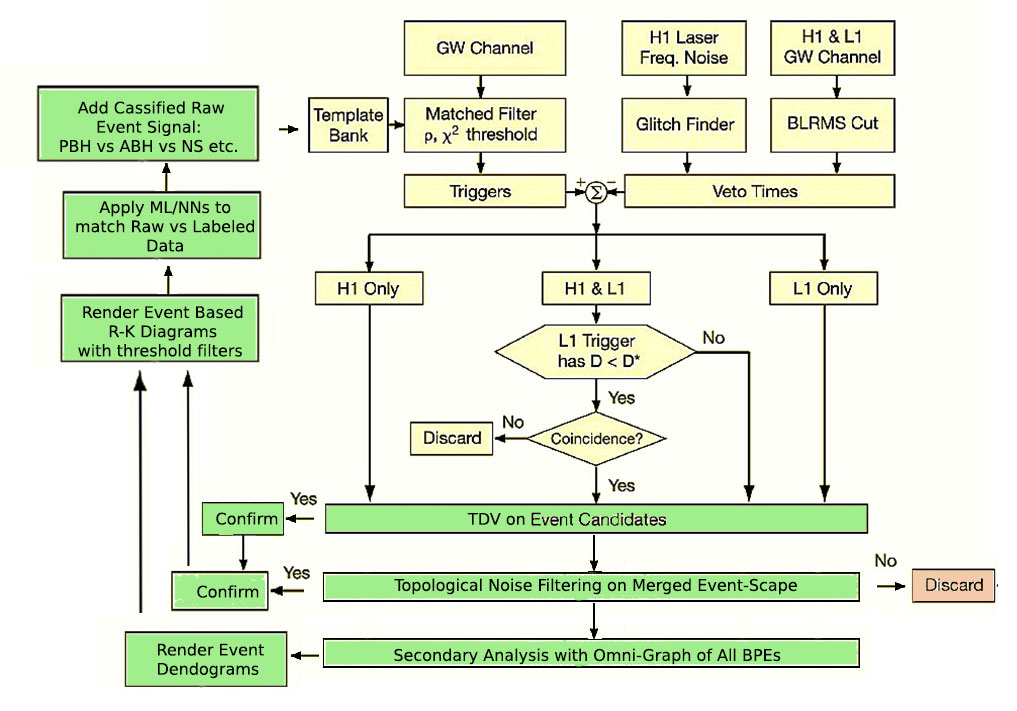
\includegraphics[width=1.0\linewidth]{images/Modified-TDA-LIGO-Analysis-Pipeline.jpg}
	\caption{\textit{Modifying and augmenting a current version of the LIGO Analysis Pipeline with
			Topology, Graph Theory \& Machine Learning based components of the R-K pipeline in future to operate near-real-time at the detector source}}
	\label{fig:odified-TDA-LIGO-Analysis-Pipeline}
\end{figure}

In the diagram above, the components marked in yellow represent the existing components of the LIGO Analysis pipeline  as established by Abbott et.al. However, the green components of the diagram represent components of the R-K pipeline that could further augment and enhance its existing capabilities in terms of gravitational wave signal identification and the automated segregation and classification of compact-binary mergers. This can be achieved through effective computational frameworks involving Topology and Graph Theory where conventional machine learning techniques and neural networks have limited scope of application as proposed in this paper. Furthermore, R-K Diagrams can not only be used to explore  interesting ways of providing compact binary merger classifications, but they can also enrich the template banks for future identification, segregation and classification of gravitational wave merger signals detected at source.

An example of such a template bank has been conceptualised in the diagram below. In this case, any tertiary analysis  parameters obtained from future research papers could be easily added to this TDA pipeline  to better classify compact binary merges. Even though each binary merger could render R-K diagrams that vary in geometry, they would have strong categorical correlation with respect to topological similarity measures demonstrated in this paper.
 

 \begin{figure}[H]
	\centering
	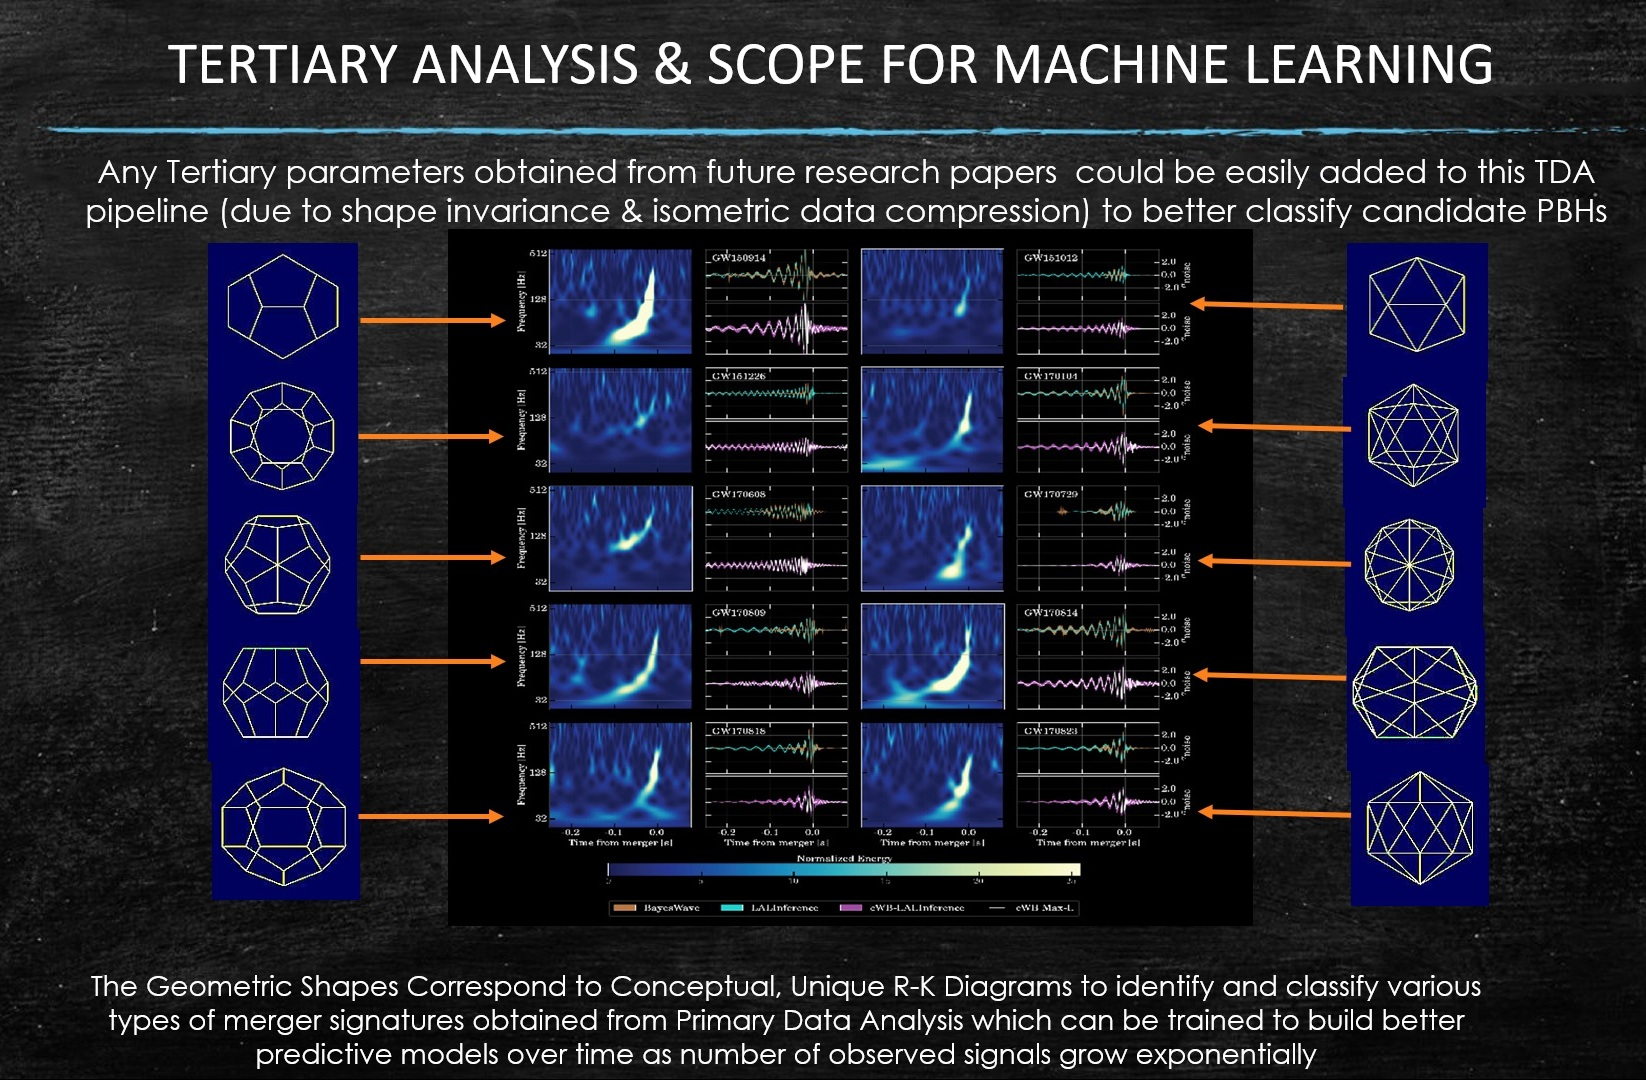
\includegraphics[width=1.0\linewidth]{images/79_Tertiary Analysis & ML Predictions.jpg}
	\caption{\textit{Binary Merger Event Classifications based on Tertiary Analysis and ML Predictions based on training of Similarity \& Divergence Measures between Topological Signatures of Merger Events }}
	\label{fig:LIGO18_PlaceHolder_fig}
\end{figure}

In the above diagram, the geometric shapes correspond to conceptual, unique R-K Diagrams to identify and classify various types of merger signatures obtained from Primary Data Analysis which can be trained to build better predictive models over time as number of observed signals grow exponentially along with the addition of new parameters to R-K models using Multi-messenger data-streams. 


\subsection{Results \& Discussions}

Thus, the LIGO case study has clearly demonstrated the validity of this novel approach to Topological Graph Theory using R-K diagrams by providing a robust, flexible and scalable computational framework for the purpose of gravitational wave detector signal identification and compact binary merger classifications. It addresses some of the existing challenges with respect to the analysis of low mass-low spin compact binary mergers pertaining to Neutron Stars and candidate Primordial Black Holes by addressing the topological similarity and divergence across classes with effective ways of addressing computational complexity. It also provides an automated classification framework where conventional methods using machine learning and neural networks fall short due to lack of training data and limitations in terms of optimizing loss on multiple high dimensional data parameters all at once. One of the most unique advantages of this novel approach using R-K diagrams lies in ability to extract ontology driven effective summaries from high dimensional datasets containing significant amount of noise. it is also able to reduce analytical complexities significantly by providing a coordinate independent framework in phase space where discreet similarity or divergence measures can be obtained by varying changes on multiple data parameters all at once. Thereby it reduces complex classification problems to topological similarity and divergence measures as a measure of overall distance between any 2 R-K diagrams or their corresponding clusters in topological phase space. It can also enrich template banks for future predictive modelling on raw/primary gravitational wave data obtained from detectors at source and could effectively scale to include all multi-messenger data-streams to provide meaningful data summaries using R-K models and filtered, compressible R-K diagrams. Thus, novel techniques such as this could be eventually used to gain unique perspectives on all of Dark Matter using Multi-Messenger data sources in the near future.
